% Chapter Template

\chapter{Diseño e Implementación} % Main chapter title

\label{Chapter3} % Change X to a consecutive number; for referencing this chapter elsewhere, use \ref{ChapterX}
En el siguiente capítulo se presenta el diseño y la implementación de las tres partes fundamentales del equipo. Se abarcan aspectos de diseño de hardware, desarrollo de firmware y diseño y fabricación mecánica.
%----------------------------------------------------------------------------------------
%	SECTION 1
%----------------------------------------------------------------------------------------

\definecolor{mygreen}{rgb}{0,0.6,0}
\definecolor{mygray}{rgb}{0.5,0.5,0.5}
\definecolor{mymauve}{rgb}{0.58,0,0.82}
%%%%%%%%%%%%%%%%%%%%%%%%%%%%%%%%%%%%%%%%%%%%%%%%%%%%%%%%%%%%%%%%%%%%%%%%%%%%%
% parámetros para configurar el formato del código en los entornos lstlisting
%%%%%%%%%%%%%%%%%%%%%%%%%%%%%%%%%%%%%%%%%%%%%%%%%%%%%%%%%%%%%%%%%%%%%%%%%%%%%
\lstset{ %
  backgroundcolor=\color{white},   % choose the background color; you must add \usepackage{color} or \usepackage{xcolor}
  basicstyle=\footnotesize,        % the size of the fonts that are used for the code
  breakatwhitespace=false,         % sets if automatic breaks should only happen at whitespace
  breaklines=true,                 % sets automatic line breaking
  captionpos=b,                    % sets the caption-position to bottom
  commentstyle=\color{mygreen},    % comment style
  deletekeywords={...},            % if you want to delete keywords from the given language
  %escapeinside={\%*}{*)},          % if you want to add LaTeX within your code
  %extendedchars=true,              % lets you use non-ASCII characters; for 8-bits encodings only, does not work with UTF-8
  %frame=single,	                % adds a frame around the code
  keepspaces=true,                 % keeps spaces in text, useful for keeping indentation of code (possibly needs columns=flexible)
  keywordstyle=\color{blue},       % keyword style
  language=[ANSI]C,                % the language of the code
  %otherkeywords={*,...},           % if you want to add more keywords to the set
  numbers=left,                    % where to put the line-numbers; possible values are (none, left, right)
  numbersep=5pt,                   % how far the line-numbers are from the code
  numberstyle=\tiny\color{mygray}, % the style that is used for the line-numbers
  rulecolor=\color{black},         % if not set, the frame-color may be changed on line-breaks within not-black text (e.g. comments (green here))
  showspaces=false,                % show spaces everywhere adding particular underscores; it overrides 'showstringspaces'
  showstringspaces=false,          % underline spaces within strings only
  showtabs=false,                  % show tabs within strings adding particular underscores
  stepnumber=1,                    % the step between two line-numbers. If it's 1, each line will be numbered
  stringstyle=\color{mymauve},     % string literal style
  tabsize=2,	                   % sets default tabsize to 2 spaces
  title=\lstname,                  % show the filename of files included with \lstinputlisting; also try caption instead of title
  morecomment=[s]{/*}{*/}
}

\section{Hardware}
\label{section:Hardware}
\subsection{Diseño basado en módulos de hardware libre}
\label{subsection:Diseño basado en módulos de hardware libre}

El diseño de la placa electrónica se basó en el estudio de los siguientes módulos:
\begin{itemize}
\item TMC5130-EVAL \citep{3_web_trinamic_placa}	
\item NodeMCU \citep{web_nodemcu}
\end{itemize}
Se destaca que ambos proyectos adhieren a la filosofía del hardware libre. Por lo tanto se pudieron descargar y estudiar los diagramas esquemáticos de ambas placas. Las primeras pruebas de implementación de hardware se realizaron interconectando ambos módulos como puede observarse en la figura \ref{fig:esp_tmc5130}.

\begin{figure}[!h]
	\centering
	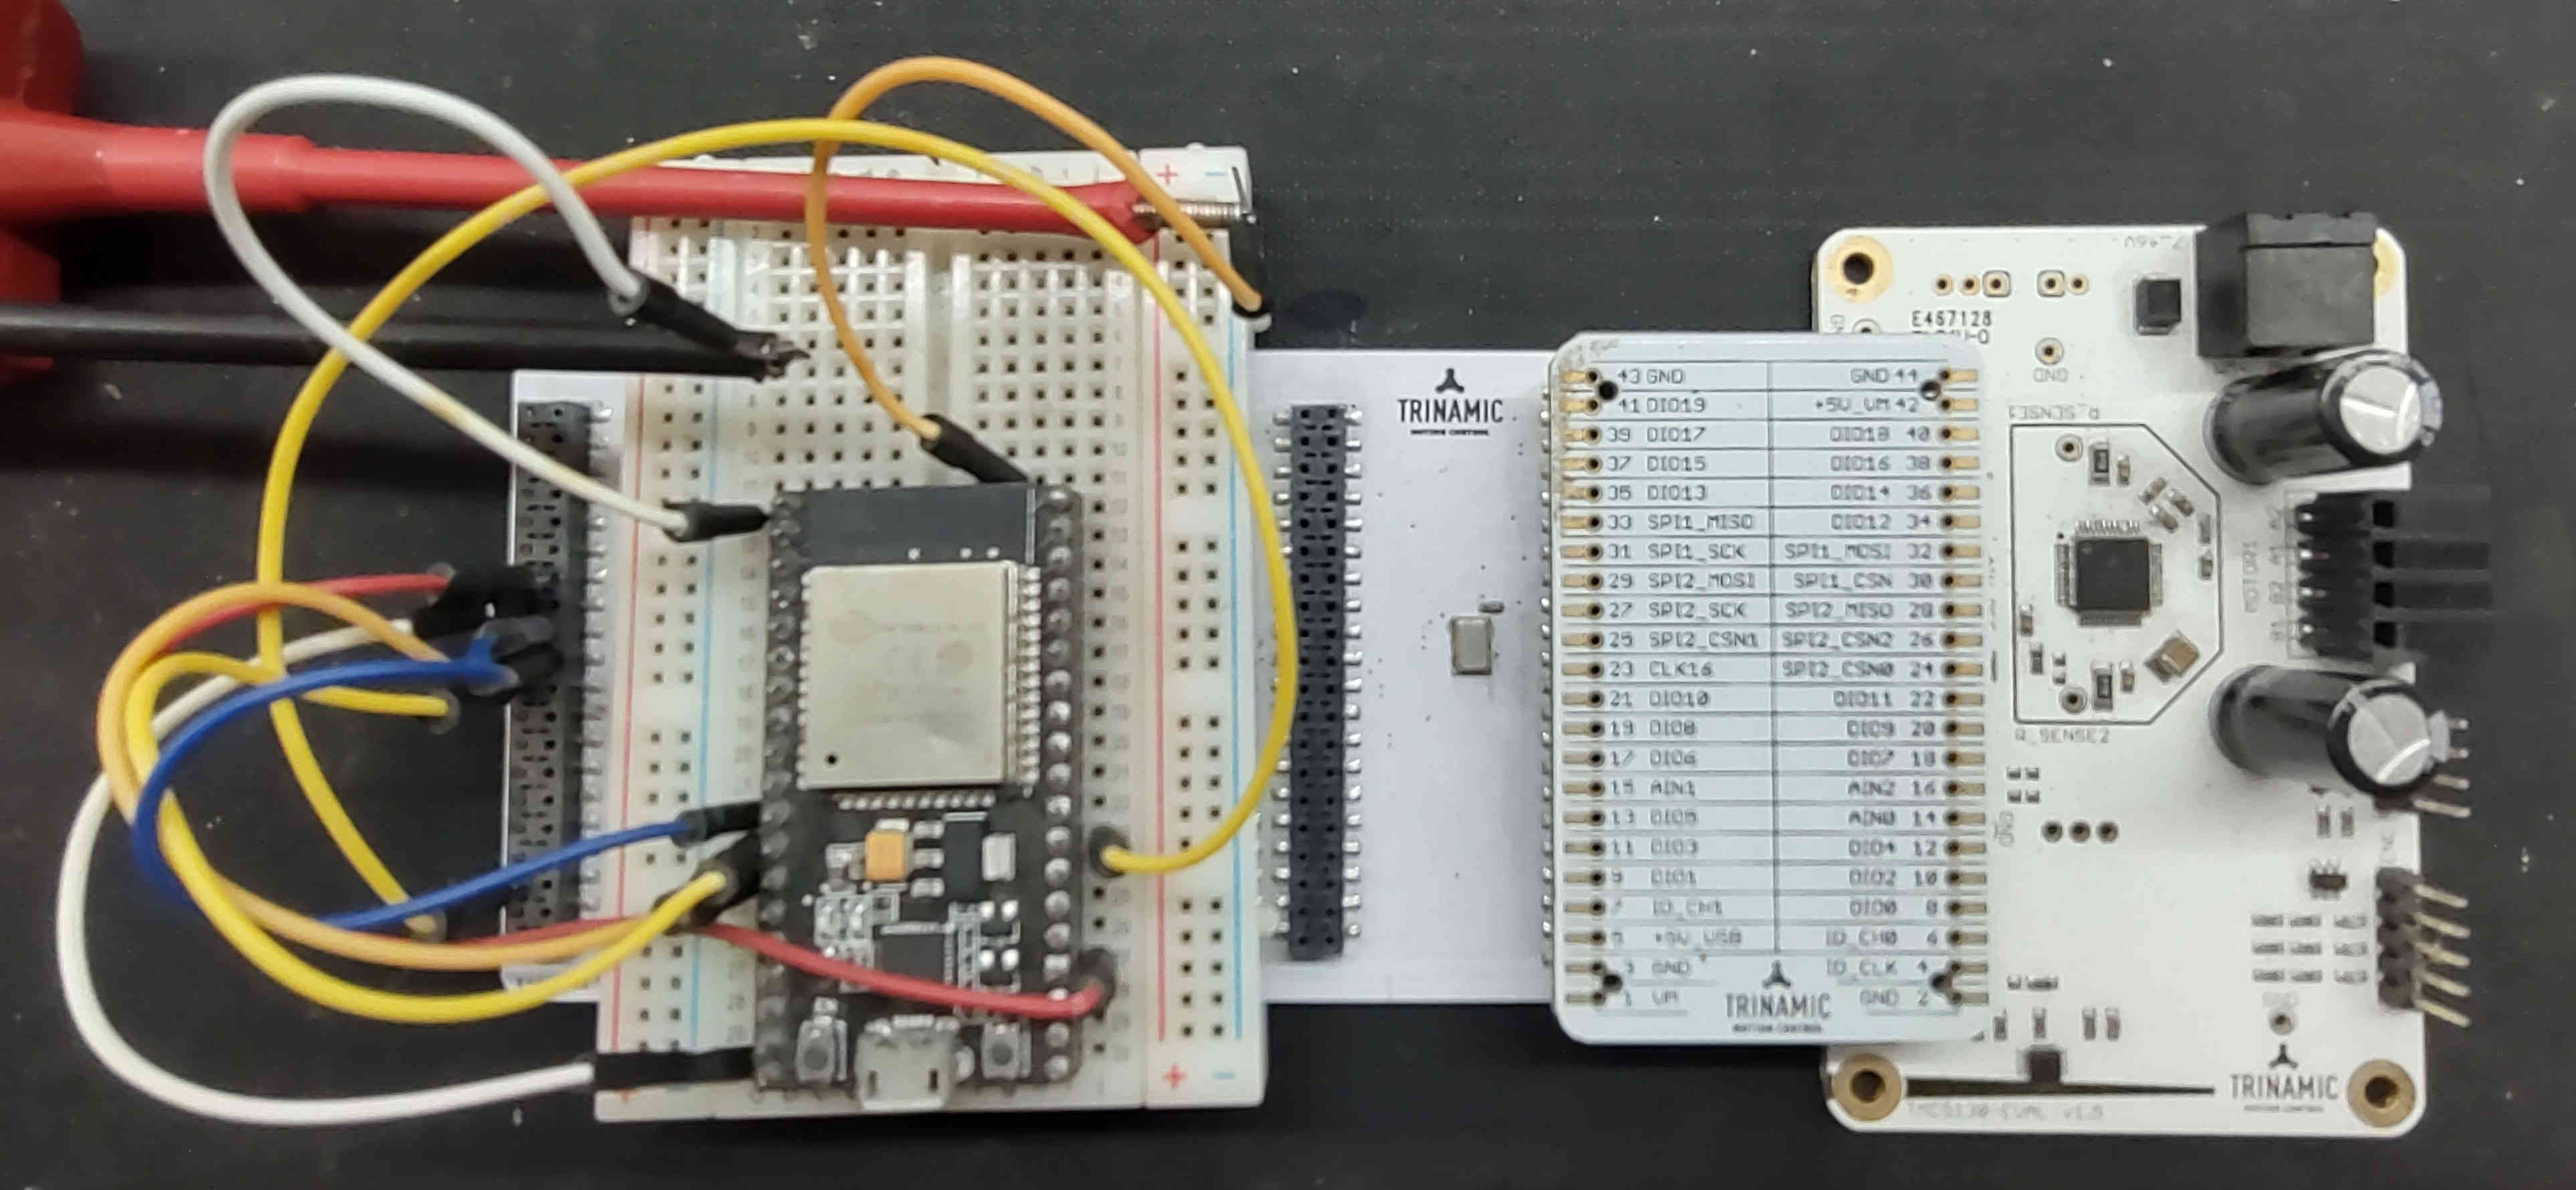
\includegraphics[width=1\textwidth]{./Figures/esp_tmc5130_v2.jpg}
	\caption{Módulo NodeMCU + TMC5130-EVAL.}
	\label{fig:esp_tmc5130}
\end{figure}

\subsection{Etapa de alimentación}

Se observa en la figura \ref{fig:kicad_tension} la etapa reguladora de tensión que permite alimentar al equipo con tensiones continuas de entre 24 V y 46 V. En el diseño se utilizó el CI LM5161 en modo \textit{step-down buck converter}, una configuración que permite bajar la tensión de entrada según la relación de las resistencias de \textit{feedback}. En este caso se configuró una salida de 5 V la cual tiene una eficiencia energética de 86 \% según su hoja de datos. Luego a través de un regulador de tensión se obtienen 3,3 V que se utilizan para alimentar el microcontrolador.

\begin{figure}[h!]
	\centering
	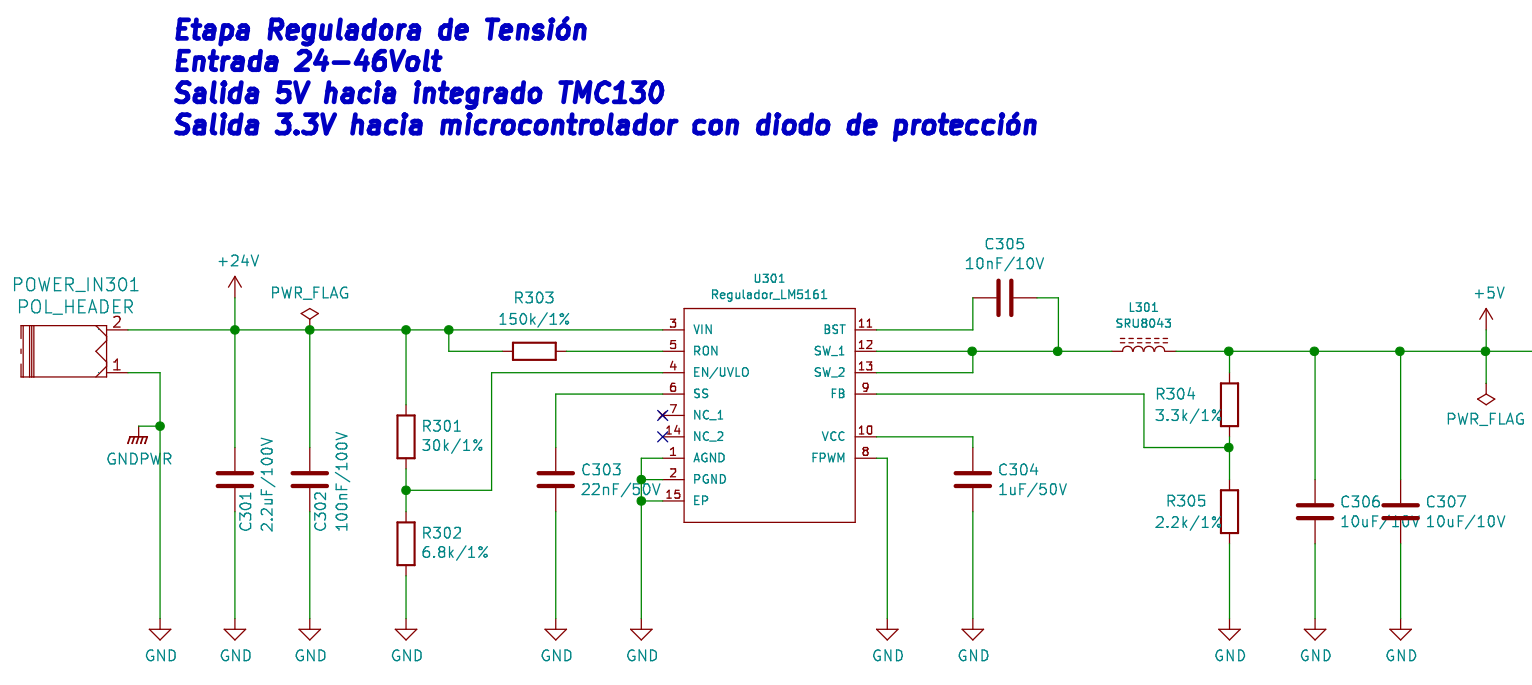
\includegraphics[width=1\textwidth]{./Figures/kicad_tension_v2.png}
	\caption{Módulo de entrada.}
	\label{fig:kicad_tension}
\end{figure}
  
El equipo se diseñó para ser alimentado con una fuente externa de tensión continua, simplificando así cuestiones regulatorias de certificación que deben cumplir equipos que se alimentan directamente de la red eléctrica.

\subsection{Etapa de comunicación}

El módulo NodeMCU es una placa de desarrollo que contiene el SoC ESP32-WROOM. A partir del estudio de su diseño, se implementó la etapa de conversión SERIAL-USB que puede observase en la figura \ref{fig:kicad_conversor}. 


\begin{figure}[h!]
	\centering
	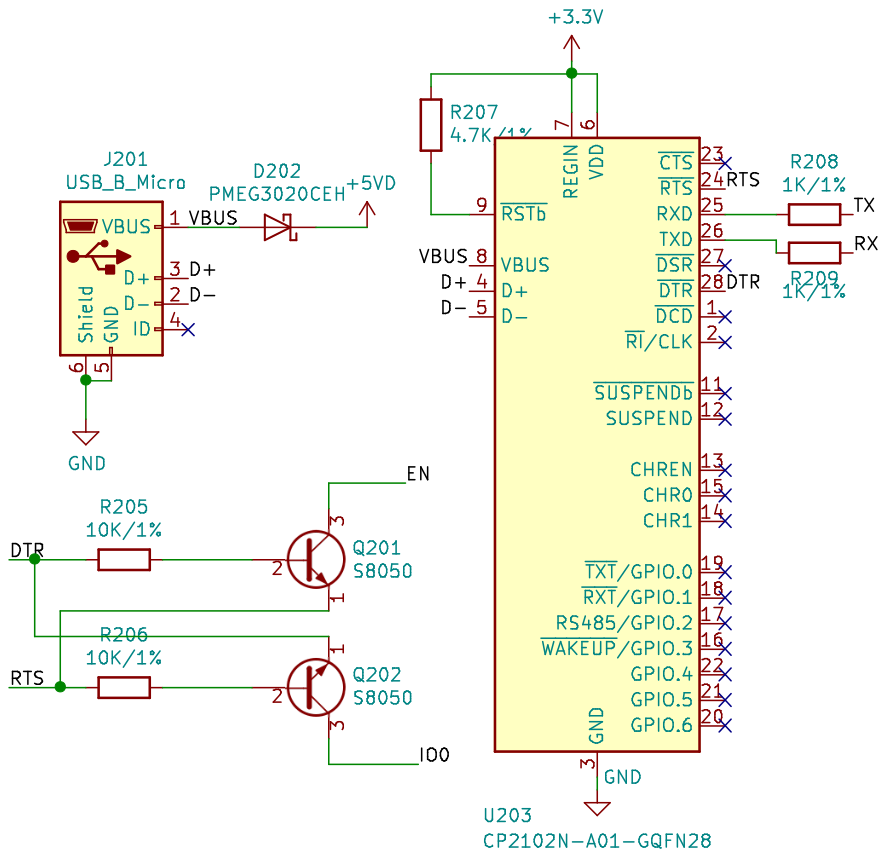
\includegraphics[width=0.6\textwidth]{./Figures/kicad_conversor_v1.png}
	\caption{Conversor serie-USB.}
	\label{fig:kicad_conversor}
\end{figure}

Mantener esta etapa de entrada en la placa electrónica final habilita la conexión directa del equipo dip coater con un puerto USB de computadora, lo cual permite establecer una comunicación constante con el periférico UART y descargar un firmware nuevo sin tener que contar con un programador externo. Se utilizó para esta etapa de conversión el CI CP2102.

Para descargar un firmware en el microcontrolador ESP32 se debe seguir la siguiente secuencia:
\begin{enumerate}
\item Mantener la terminal IO0 en GND.
\item Poner la terminal EN en GND para reiniciar el mismo.
\item El microcontrolador se inicia en modo \textit{boot}.
\item Enviar firmware desde el entorno de desarrollo. 
\end{enumerate}

La interfaz UART CP2102 consta de señales de transmisión y recepción de datos TX y RX. También admite las señales de control RTS/CTS, DSR/DTR y X-ON/X-OFF. Se incorporó en el diseño el uso de las terminales DTR y RTS para generar la secuencia de descarga de manera automática. Sin embargo la misma presentó cierta inestabilidad y no siempre se logró generar la secuencia correctamente, por tal motivo se implementará en la nueva versión de la placa botones para poder forzar dicha secuencia.



\subsection{Driver TMC5130}

El módulo TMC5130-EVAL, como se describió en la sección \ref{sec:Circuitos integrados Trinamic}, contiene al CI TMC5130. Del estudio de esta placa de evaluación se extrajeron las configuraciones necesarias para lograr la correcta utilización del driver. Se tuvieron en cuenta las recomendaciones de diseño establecidas por el fabricante, como por ejemplo la incorporación de un clock externo de 16 MHz, que se puede observar en la figura \ref{fig:kicad_clock} el cual es necesario en aplicaciones de alta precisión. 

\begin{figure}[h!]
	\centering
	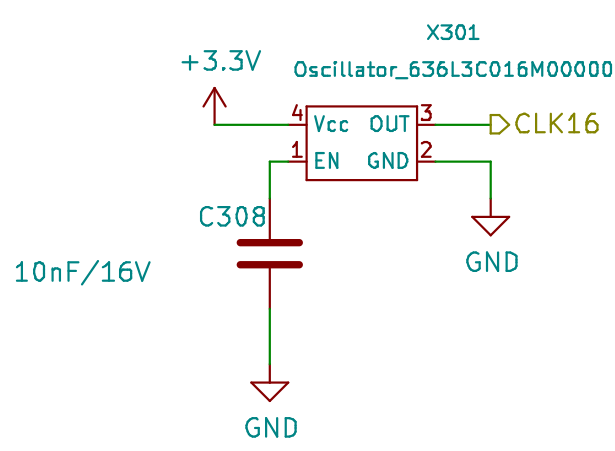
\includegraphics[width=0.5\textwidth]{./Figures/kicad_clock.png}
	\caption{Clock para el CI TMC5130.}
	\label{fig:kicad_clock}
\end{figure}



El driver se alimenta por las terminales VS/VSA con la tensión de entrada de la placa electrónica y por la terminal VCC con 5 V, los cuales son generados internamente  por un regulador en la terminal 5VOUT. Si bien esta configuración funciona, se pretende mejorar el diseño en la próxima versión de la placa. El fabricante sugiere alimentar la terminal VCC con una tensión externa para evitar el uso del regulador de tensión interno y mejorar así la eficiencia térmica del CI.

Se observa en la figura \ref{fig:kicad_trinamic} las conexiones del driver con el motor paso a paso, la etapa de alimentación y las conexiones del puerto SPI para la comunicación con el microcontrolador. 
 
\begin{figure}[h!]
	\centering
	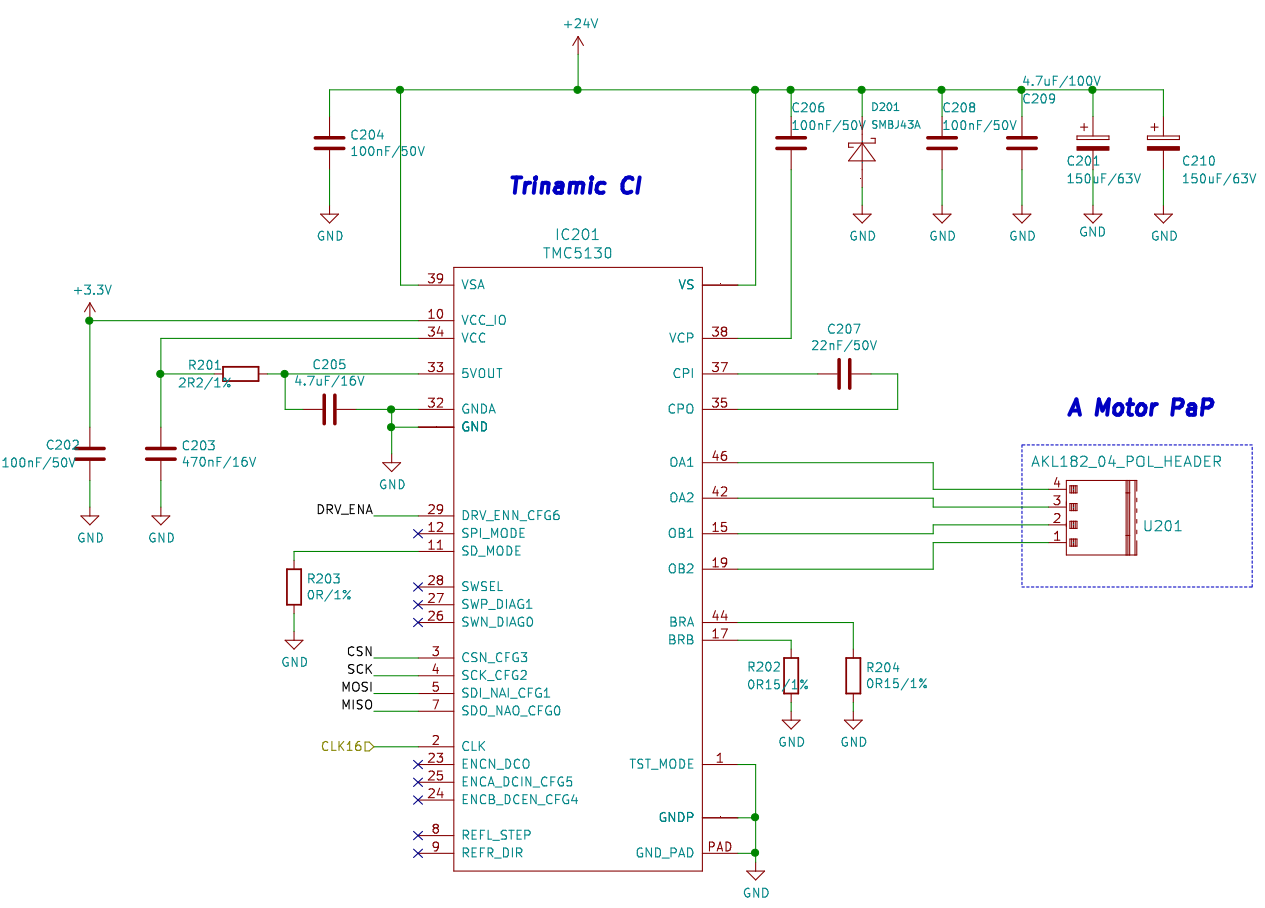
\includegraphics[width=1\textwidth]{./Figures/kicad_trinamic.png}
	\caption{CI TMC5130.}
	\label{fig:kicad_trinamic}
\end{figure} 

%\begin{figure}[h]
%	\centering
%	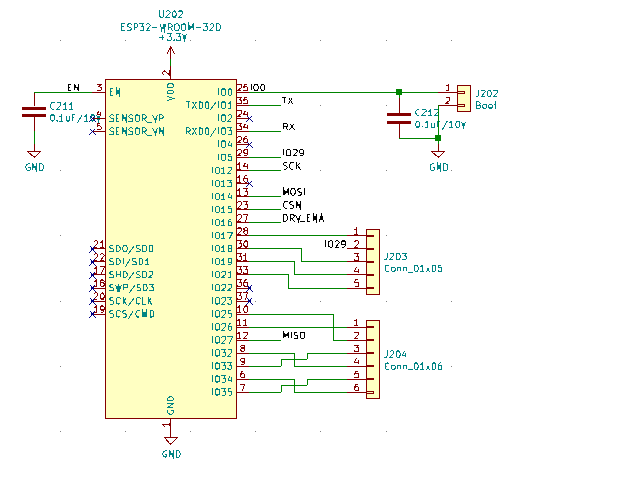
\includegraphics[width=.6\textwidth]{./Figures/kicad_esp.png}
%	\caption{Módulo ESP32.}
%	\label{fig:kicad_esp}
%\end{figure}
  
\subsection{Diseño final}  
Finalmente, se observa en la figura \ref{fig:dip_3d_model} el diseño 3D generado por el software KICAD.

Todo el diseño y material asociado se encuentra disponible en el repositorio de la empresa TECSCI \citep{web_hardware_tecsci}. La placa electrónica de este equipo dip coater cuenta con una licencia CERN OHL v.1.2 \citep{web_cern_licence}.


\begin{figure}[h!]
	\centering
	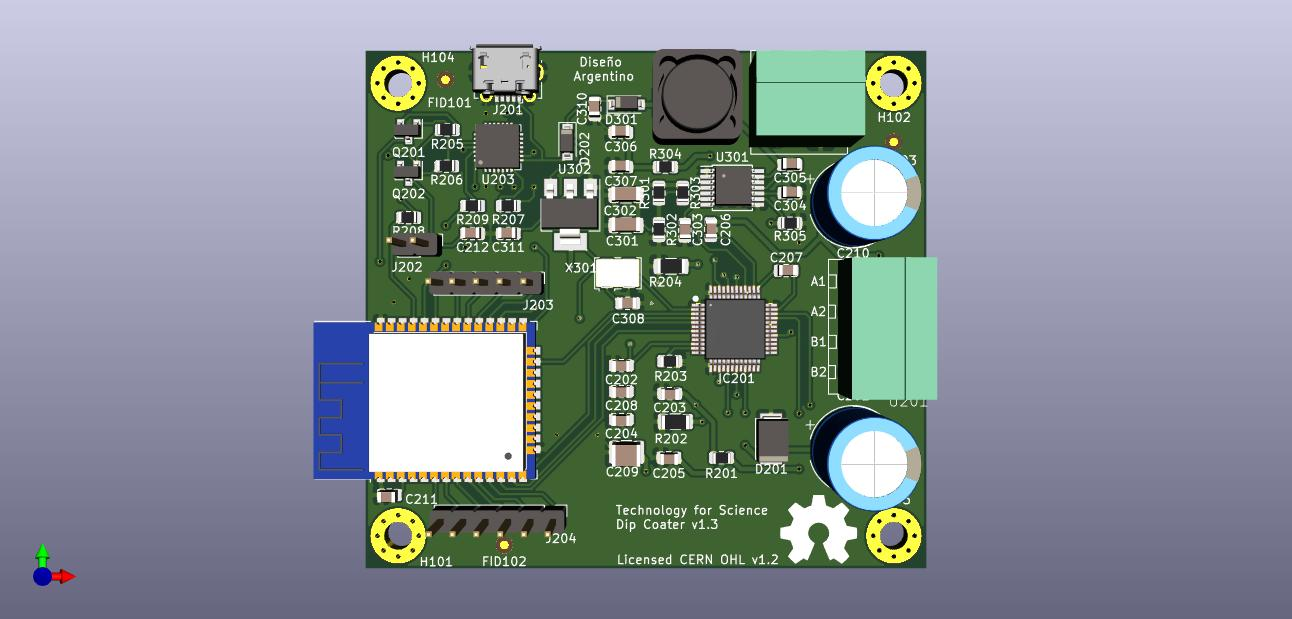
\includegraphics[width=1\textwidth]{./Figures/tecsci_dip.jpg}
	\caption{Modelo 3D Kicad.}
	\label{fig:dip_3d_model}
\end{figure}
         



  
%-----------------------------------
%	SUBSECTION 1
%-----------------------------------
\subsection{Fabricación}
%-----------------------------------
%	SUBSECTION 2
%-----------------------------------
La placa electrónica se fabricó con el proveedor local de circuitos impresos Ernesto Mayer S.A. \citep{web_mayer}. A continuación se presenta la información de diseño de la misma y se describen  restricciones impuestas por el propio fabricante:

\begin{itemize}

\item Grilla de posicionamiento principal: 0,25 mm.
\item Grilla de ruteo principal: 0,25 mm.
\item Agujeros de montaje: 3,2 mm.
\item Pistas principales: 0,5 mm.
\item Pistas inferiores: 0,25 mm, con límite particular 0,20mm (8 mils).
\item Pistas superiores: 0,8 mm.
\item Vías: 0,8 mm /0,4 mm, con límite particular 0,20mm (8 mils).
\item Margen general: 0,22 mm.
\item Margen particular: 0,2 mm, con límite particular 0,20 mm (8 mils).
\item Fabricación: espesor 1,6mm FR4.  
\item Restricciones generales del fabricante: con límite estándar 0,254 mm (10 mils).

\end{itemize}

Luego de fabricar el PCB, se continuó con el montaje de componentes electrónicos superficiales, que estuvo a cargo de la empresa Asembli S.A. \citep{web_asembli}. Se fabricó un primer lote de cinco placas. En la figura \ref{fig:dip_real_model} se observa la placa con los componentes montados.


\begin{figure}[htbp]
	\centering
	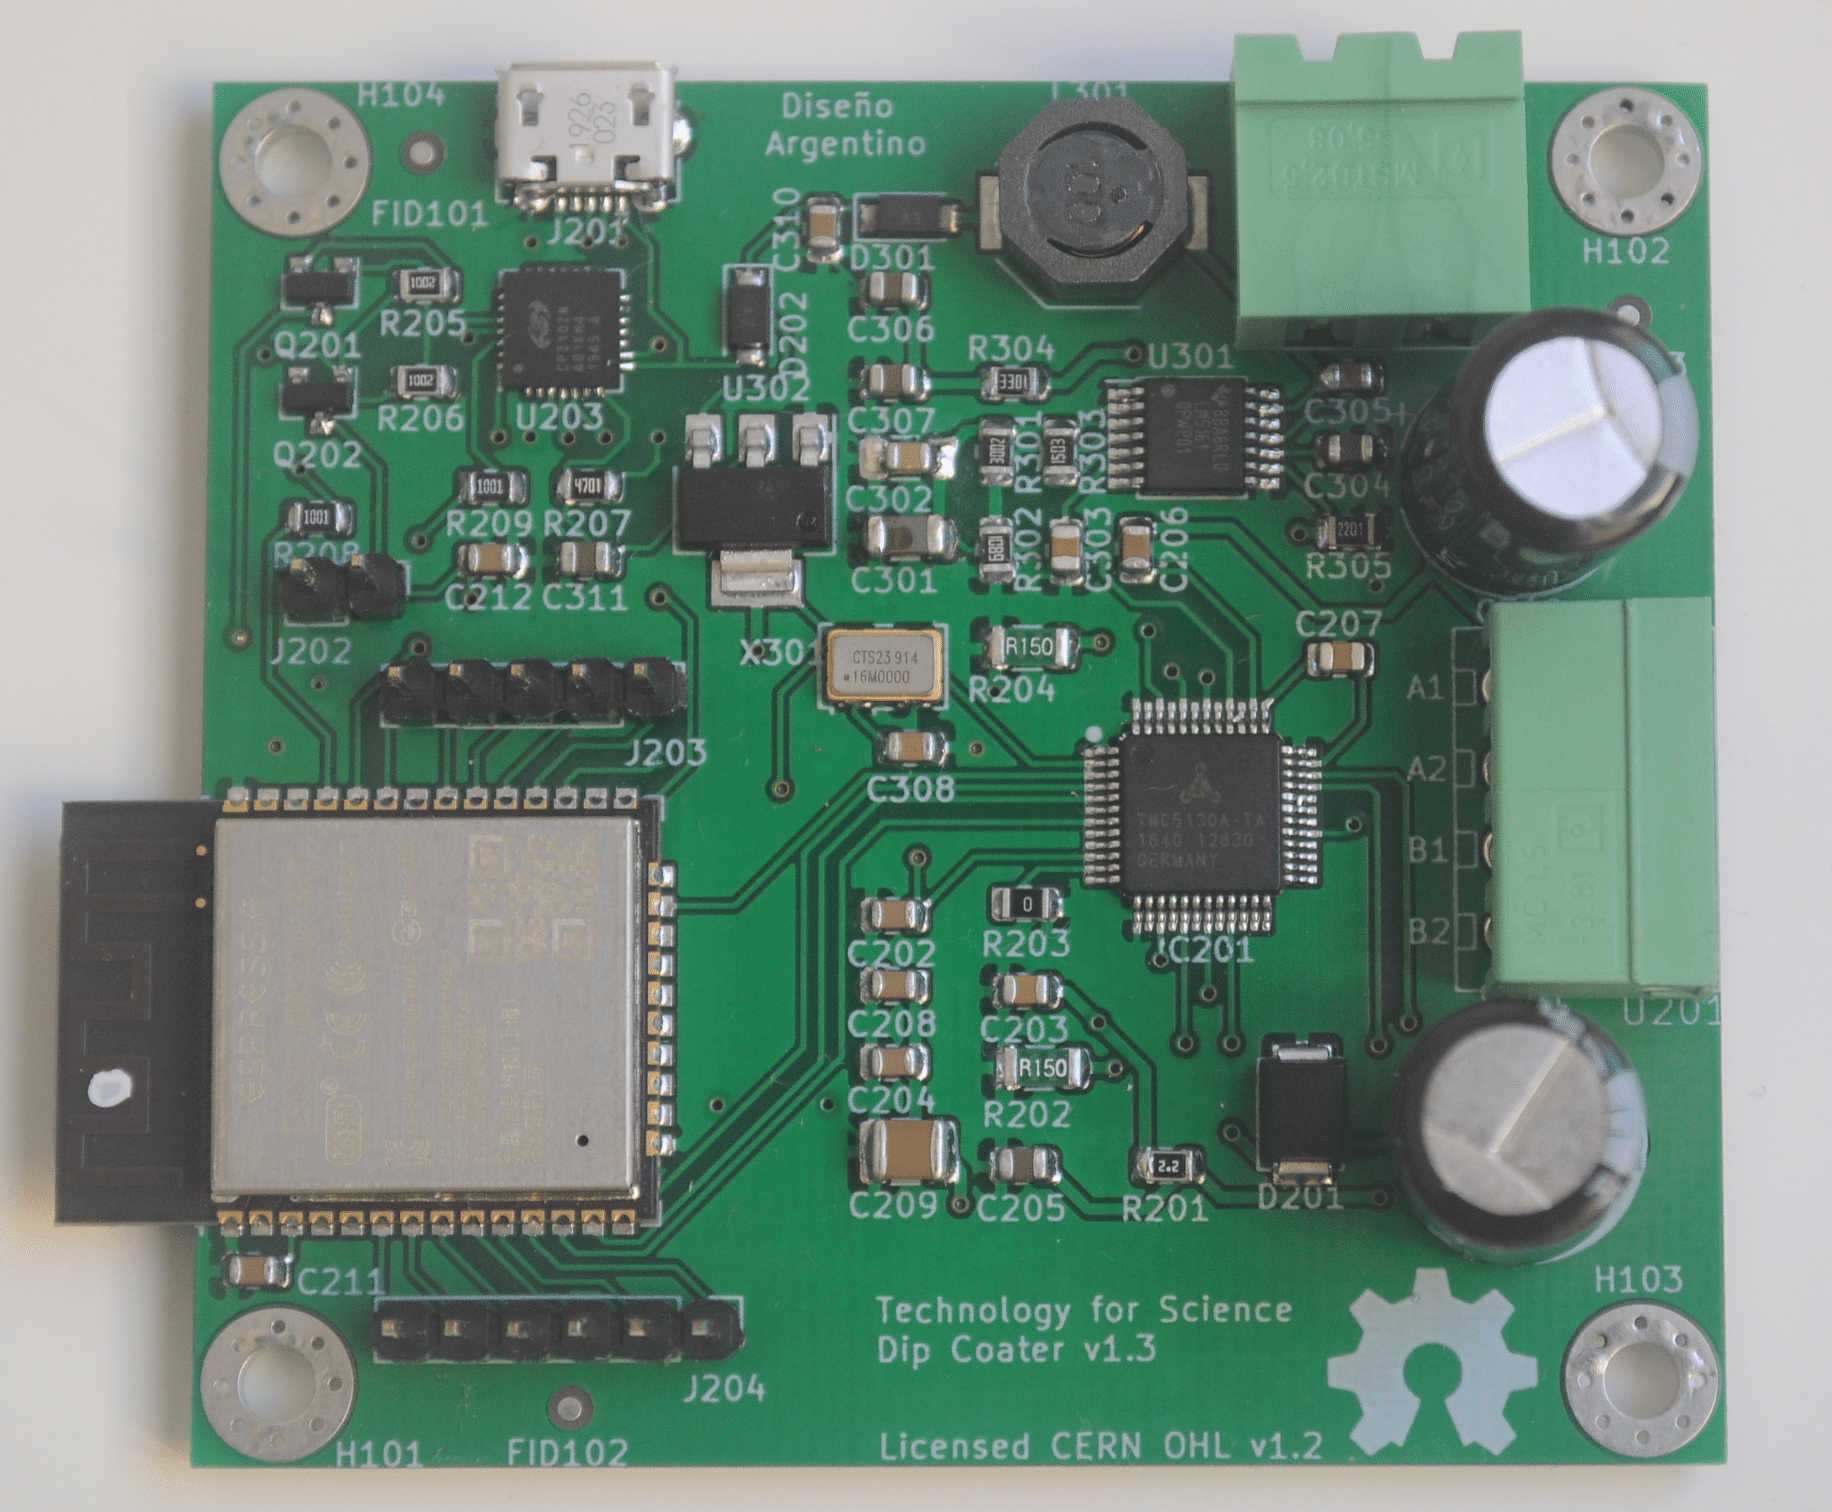
\includegraphics[width=0.6\textwidth]{./Figures/dip_real_model.jpg}
	\caption{Plaqueta electrónica final.}
	\label{fig:dip_real_model}
\end{figure}

%----------------------------------------------------------------------------------------
%	SECTION 2
%----------------------------------------------------------------------------------------

\section{Firmware}
\subsection{Capas de abstracción}

Se desarrolló un firmware modular que permite incorporar código de manera incremental y ordenada. Se observan en la figura \ref{fig:capas} las capas de abstracción de software implementadas. Esta solución tiene dos ideas fundamentales:

\begin{itemize}
\item No permitir llamados a funciones entre capas discontinuas. Los módulos de la capa superior o capa APP solo pueden hacer llamados a funciones de la capa intermedia o capa API \textit{(Application Programming Interfaces)} y estas últimas solo pueden llamar a funciones de la capa inferior o capa BOARD.
\item Las aplicaciones funcionan de manera independiente, las mismas se pueden habilitar o deshabilitar individualmente.
\end{itemize}

\begin{figure}[h]
	\centering
	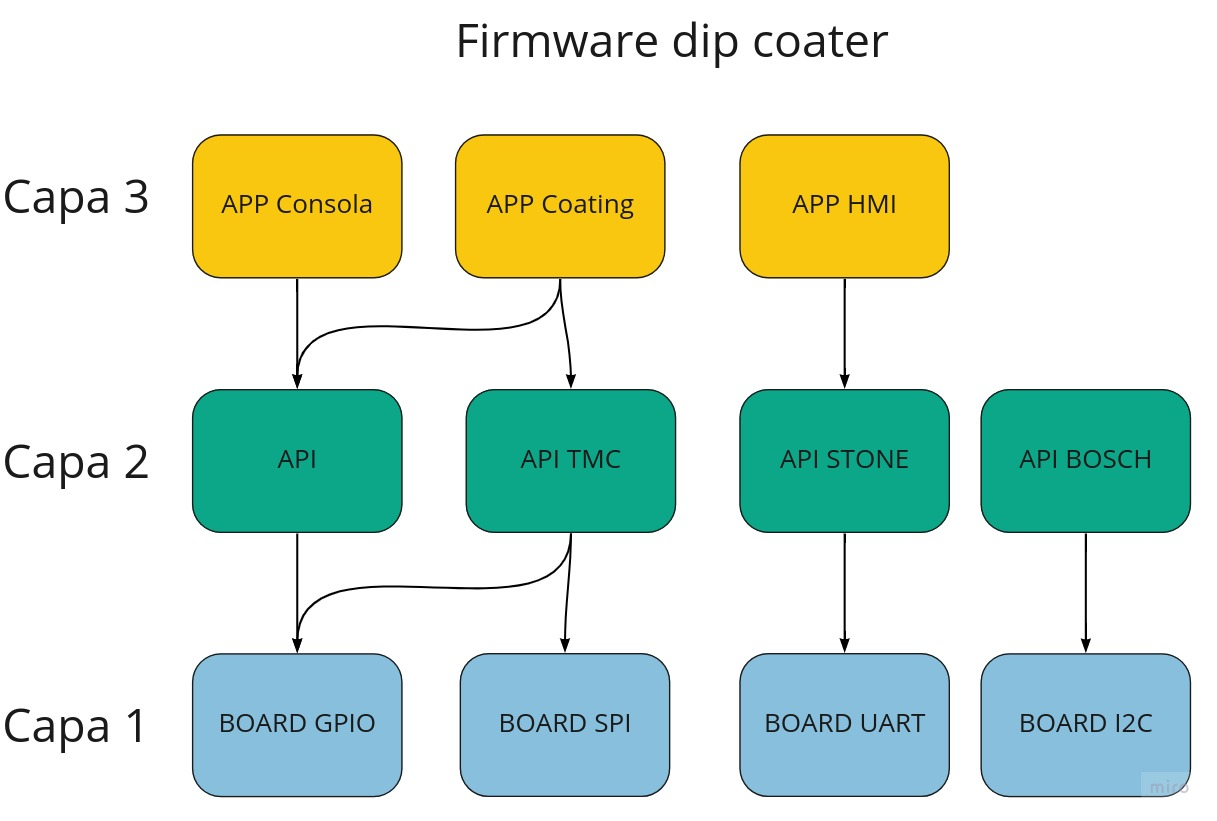
\includegraphics[width=1\textwidth]{./Figures/capas.jpg}
	\caption{Capas de abstracción de software.}
	\label{fig:capas}
\end{figure}


La capa tres corresponde a la capa de aplicaciones. El firmware cuenta con 3 aplicaciones fundamentales para el funcionamiento del equipo y una aplicación de testing utilizada para probar nuevos componentes de software. Cada aplicación contiene al menos una \textit{task} del sistema operativo freeRTOS. A continuación se detallan las aplicaciones:

\begin{itemize}

\item APP coating: se encarga de la comunicación con el driver TMC5130, de la ejecución de movimientos individuales y del proceso completo de dip coating.
\item APP consola: administra una consola de comandos que permite ejecutar y configurar el equipo a través de una comunicación serial. Recibe y procesa comandos de la consola y los envía a través de una \textit{queue} de freeRTOS a la app coating.
\item APP hmi: administra la interfaz de configuración, establece una comunicación serial con la pantalla táctil, recibe comandos a través de una \textit{queue} de freeRTOS y los envía a la app coating para ser procesados.
\item APP test: se utiliza para probar nuevos componentes y realizar \textit{test} sobre el sistema.

\end{itemize}
% y realizar test sobre el sistema que se activa y desactiva según la necesidad de uso.

La capa dos esta compuesta por bloques de código provistos por los fabricantes de drivers:
\begin{itemize}
\item API TMC: provista por el fabricante Trinamic y adaptada para ser ejecutada bajo el framework ESP-IDF.
\item API BOSH: provista por el fabricante y adaptada a este firmware.
\item API STONE: contiene los módulos de software que interaccionan con la pantalla táctil.
\item API: se utiliza como puente hacia la capa BOARD que tiene acceso a los periféricos del microcontrolador y con módulos de software del \textit{framework} ESP-IDF.

\end{itemize}

La capa uno es la que interacciona con los módulos de hardware del microcontrolador. Por lo tanto, esta capa es la única que contiene llamados a funciones disponibles en el framework ESP-IDF, como por ejemplo las funciones de configuración de los periféricos UART, GPIO, SPI, etc. Es importante mencionar que si debido a un rediseño se decide cambiar el microcontrolador utilizado, solo se deberán reescribir los módulos pertenecientes a esta capa y se podrá mantener el resto del programa sin alteraciones.

\subsection{Módulos principales de software}
\label{sec:modulos principales}

\subsubsection{Funcionamiento general}
 

El equipo dip coater puede ser utilizado de dos maneras diferentes:

\begin{enumerate}
\item A través de una consola de comandos.
\item A través de una pantalla táctil.
\end{enumerate}

Ambas opciones permiten ejecutar un ciclo completo de dip coating y también permiten ejecutar comandos de manera individual. Las aplicaciones app consola y app hmi se encargan de la interacción con el usuario y son las encargadas de enviar a la aplicación app coating los comandos para ejecutar los distintos movimientos.

\subsubsection{Control de movimientos}

La aplicación app coating contiene toda la lógica de control de movimientos. La misma se encarga de realizar la configuración inicial del driver TMC5130, de ejecutar los procesos completos de dip coating y de procesar comandos individuales para generar diferentes tipos de acciones. 

Como se mencionó en la subsección \ref{subsection:Driver TMC5130} calcular los parámetros iniciales del driver es una tarea compleja, por lo que se optó por utilizar el software TMCL-IDE provisto por el fabricante y realizar la configuración de los registros de manera interactiva.

%Como se mencionó en la subsección \ref{subsection:Driver TMC5130} la configuración inicial del driver es compleja, por tal motivo se utilizo el software  TMCL-IDE provisto por el fabricante para obtener los valores de inicialización de los registros de manera interactiva.
%Cabe destacar que con este software se pueden configurar todos los driver que la compañía ofrece, abarcando desde motores paso a paso hasta  servomotores, motores \textit{brushless} y de corriente continua. 

En esta etapa de configuración es recomendable que el motor este acoplado al eje lineal, junto con el tornillo, la tuerca y el carro ya que el driver registra la corriente que circula por las bobinas del motor y calcula la fuerza contraelectromotriz que el eje esta ejerciendo. 
En la figura \ref{fig:tmcl_ide} se observa el entorno de desarrollo TMCL-IDE.  

\begin{figure}[h!]
	\centering
	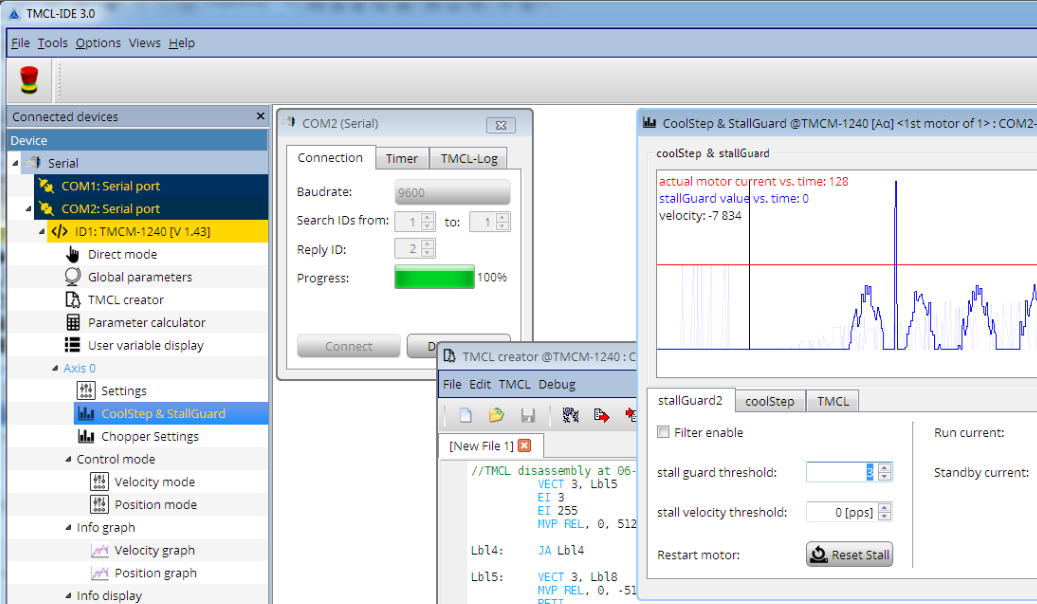
\includegraphics[width=0.8\textwidth]{./Figures/tmcl_ide_1.png}
	\caption{Software TMCL-IDE.}
	\label{fig:tmcl_ide}
\end{figure}


En la figura \ref{fig:tmcl_ide_stall} se puede observar el \textit{wizard} de configuración de las funciones \textit{stallguard2} y \textit{coolstep}.
Como se mencionó en el capítulo \ref{Chapter2} es posible usar stallguard2 para detectar los límites mecánicos de recorrido. El parámetro \textit{stall guard threshold} relaciona la fuerza contraelectromotriz registrada por el driver. A medida que se detecta mayor fuerza, es decir mayor oposición al movimiento y mayor corriente en los motores, el valor de stallguard2 disminuye. Se debe configurar entonces un valor límite de detección para que una vez alcanzado se genere un evento.

El firmware cuenta con una función llamada mod-coating-process-cero-machine que utiliza stallguard2. Se encarga de detectar el evento que el driver envía cuando se detecta un final de carrera. La misma se encarga de parar el motor, generar un desplazamiento en sentido contrario y establecer una nueva posición. Esta función se ejecuta al encender el equipo y sirve para posicionar el carro.
 

\begin{figure}[h!]
	\centering
	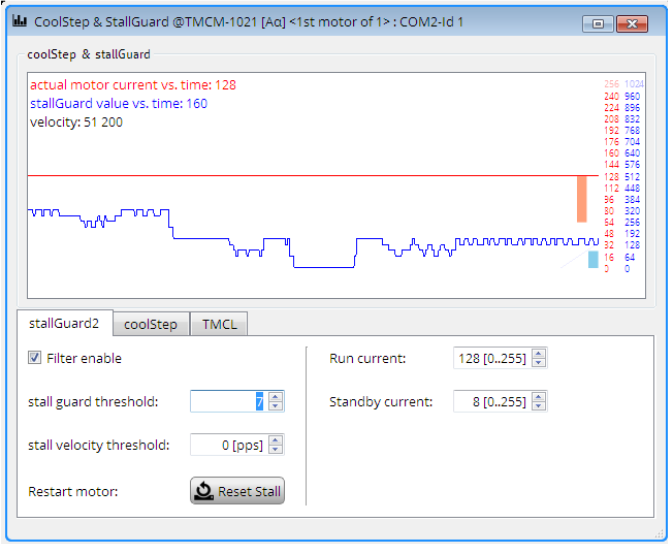
\includegraphics[width=0.6\textwidth]{./Figures/tmcl_ide_2.png}
	\caption{Configuración de funcionalidades stalldguard2 y coolstep.}
	\label{fig:tmcl_ide_stall}
\end{figure}

Otros parámetros importantes a configurar son los que definen la rampa de aceleración del desplazamiento. El driver permite configurar una rampa de seis puntos donde los valores a encontrar, A1, AMAX, D1, DMAX, V1 y VMAX corresponden a la aceleración, desaceleración y velocidad, como se observa en la figura \ref{fig:rampa}.

\begin{figure}[h!]
	\centering
	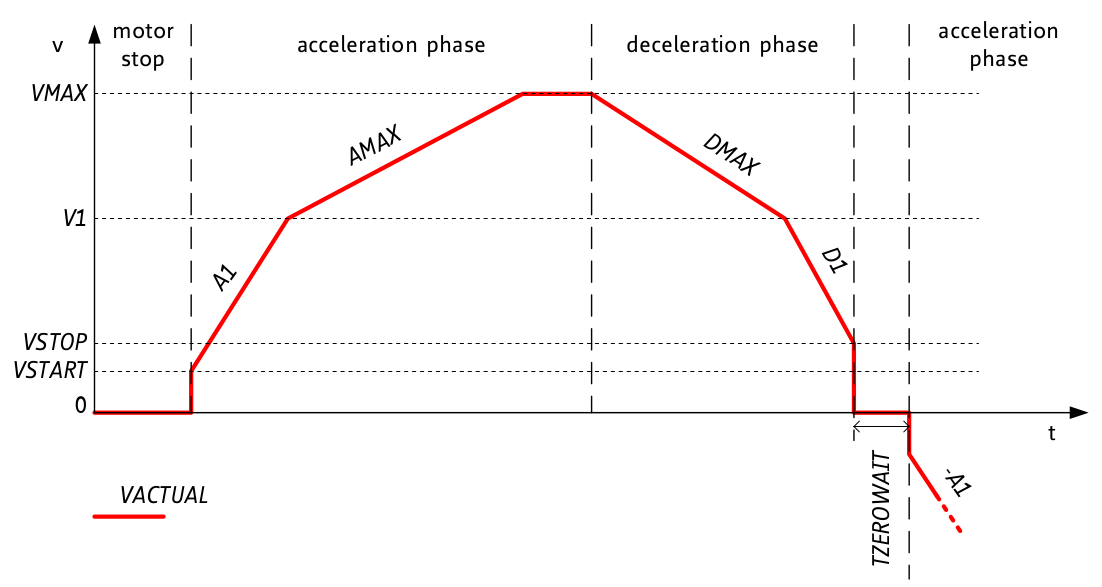
\includegraphics[width=0.8\textwidth]{./Figures/rampa_1.png}
	\caption{Configuración de rampa de seis puntos.}
	\label{fig:rampa}
\end{figure}


%Todos los movimientos del equipo dip coater están definidos de la siguiente manera \ref{cod:vControl_1}.
%\begin{lstlisting}[label=cod:vControl_1,caption=Macros para configurar de desplazamientos.] 
%	// Velocidad
%	//V1
%	Evalboards.ch1.writeRegister(0, TMC5130_V1, (arg->velocity) / 2);
%	//VMAX
%	Evalboards.ch1.writeRegister(0, TMC5130_VMAX, arg->velocity);
%	//VSTART
%	Evalboards.ch1.writeRegister(0, TMC5130_VSTART, 0);
%	//VSTOT
%	Evalboards.ch1.writeRegister(0, TMC5130_VSTOP, 100);
%
%	// Seteo Aceleracion
%	//A1
%	Evalboards.ch1.writeRegister(0, TMC5130_A1,  arg->acceleration);
%	//AMAX
%	Evalboards.ch1.writeRegister(0, TMC5130_AMAX,  arg->acceleration);
%
%	// Seteo Desaceleracion
%
%	//DMAX
%	Evalboards.ch1.writeRegister(0, TMC5130_DMAX,  arg->acceleration);
%	//D1
%	Evalboards.ch1.writeRegister(0, TMC5130_D1,  arg->acceleration);
%\end{lstlisting}

Para el control de los movimientos se optó por generar una rampa de cuatro puntos. Se implementó la siguiente relación de variables:

\begin{itemize}
\item A1 = AMAX  (Aceleración establecida por usuario).
\item D1 = DMAX  (Desaceleración establecida por usuario).
\item VMAX 	  (Velocidad establecida por usuario).
\item V1 = VMAX / 2 (Velocidad fija del movimiento).

\end{itemize}

Estas relaciones de variables están fijas en el firmware y no pueden ser cambiadas por el usuario, es decir que los movimientos del equipo siempre responden a una rampa de aceleración de cuatro puntos.


A modo de ejemplo, se presenta el fragmento de código \ref{code:vDownCode} que pertenece a la aplicación app coating y se ejecuta cuando llega un comando de movimiento individual.


\begin{lstlisting}[label=code:vDownCode,caption=Ejecución de comando DOWN.] % 

int HandlerDown_without_program(processCommandArgSpin_t*	arg) {
	int32_t reg_rampstat, position_actual , position_target;
	processDipCoating.config.status=1;
	Evalboards.ch1.enableDriver(DRIVER_ENABLE);

	//Leo Posicion Actual
	Evalboards.ch1.readRegister(0, 0x21, &position_actual);
	// Set velocidad
	//V1
	Evalboards.ch1.writeRegister(0, TMC5130_V1, (arg->velocity) / 2);
	//VMAX
	Evalboards.ch1.writeRegister(0, TMC5130_VMAX, arg->velocity);
	//VSTART
	Evalboards.ch1.writeRegister(0, TMC5130_VSTART, 0);
	//VSTOT
	Evalboards.ch1.writeRegister(0, TMC5130_VSTOP, 100);
	// Set aceleracion y desaceleracion
	//A1
	Evalboards.ch1.writeRegister(0, TMC5130_A1,  arg->acceleration);
	//AMAX
	Evalboards.ch1.writeRegister(0, TMC5130_AMAX,  arg->acceleration);
	// Seteo desaceleracion
	//DMAX
	Evalboards.ch1.writeRegister(0, TMC5130_DMAX,  arg->acceleration);
	//D1
	Evalboards.ch1.writeRegister(0, TMC5130_D1,  arg->acceleration);

	/* Seteo de registro XTARGET*/
	position_target=position_actual+arg->displacement_z;
	position_target = mod_coating_handlers_control_limit_(position_target);
	Evalboards.ch1.writeRegister(0, TMC5130_XTARGET, position_target);

		/*Detecto el flag que detecta XACTUAL=XTARGET y apago driver*/
	while (1 == processDipCoating.config.status) {
		Evalboards.ch1.readRegister (0, TMC5130_RAMPSTAT, &reg_rampstat);
		/*Leo registro y comparo, velocidad zero  y  position_actual == position_target */
		if (reg_rampstat & 0x00000600) {
			break;
		}
		else {
			vTaskDelay (OS_CONFIG_MOD_HANDLERS_COMMANDS_TASK_PERIOD / portTICK_PERIOD_MS);
		}
	}
	vTaskDelay(OS_CONFIG_MOD_HANDLERS_COMMANDS_TASK_PERIOD_LONG / portTICK_PERIOD_MS);
	processDipCoating.config.status=0;
	Evalboards.ch1.enableDriver(DRIVER_DISABLE);

	return 0;
}
\end{lstlisting}

Se detallan a continuación las líneas más importantes:

\begin{itemize}
\item [1] Recepción de estructura de datos con valores de aceleración, velocidad y desplazamiento.
\item [4] Habilitación del driver.
\item [7] Registro de la posición actual.
\item [8-26] Carga de parámetros de velocidad y aceleración que forman rampa de cuatro puntos.
\item [29] Suma el desplazamiento deseado con la posición actual.
\item [30] Control de limites mecánicos.
\item [31] Se escribe el registro XTARGET y se da inicio al movimiento.
\item [37] Dentro de un ciclo \textit{while} se controlan dos bits del registro RAMPSTAT que se activan cuando XACTUAL = XTARGET (fin del movimiento).
\item [46] Deshabilitación del driver si se cumple la condición anterior.  
\end{itemize}


Otra parte importante de app coating es la definición del proceso completo de dip coating, el mismo está implementado con un arreglo de estructuras de tamaño fijo. Cada item del arreglo esta compuesto por el tipo de movimiento, los valores de parámetros que se reciben desde app consola o app hmi y punteros a funciones que ejecutan cada movimiento. Es decir que el proceso completo de dip coating está formado por una concatenación de movimientos individuales, como puede observarse en el siguiente fragmento de código \ref{cod:vEstructuraCode}.

\begin{lstlisting}[label=cod:vEstructuraCode,caption=Proceso completo de dip coating.] % 

processCommand_t cmdProcessCustom[MAX_ESTATIC_COMMAND] = {

/*Deplazamiento hasta muestra*/
{ .commandnumber = PROCESS_COMMAND_DOWN, 		 	.fp = HandlerDownUntil},
{ .commandnumber = PROCESS_COMMAND_WAIT, 			.fp = HandlerWait},
/*Comienzo de ciclo*/
{ .commandnumber = PROCESS_COMMAND_DOWN, 		  .fp = HandlerDownLoop },
{ .commandnumber = PROCESS_COMMAND_WAIT, 			.fp = HandlerWaitDown },
{ .commandnumber = PROCESS_COMMAND_UP, 			 	.fp = HandlerUpLoop },
{ .commandnumber = PROCESS_COMMAND_WAIT, 			.fp = HandlerWaitUp },
/*Fin de ciclo */
{ .commandnumber = PROCESS_COMMAND_FINISH,		.fpcommandhandler = HandlerFinish},
}; 

\end{lstlisting}

Esta implementación es fija en el firmware pero se puede modificar con facilidad. Surgió en charlas con investigadores usuarios de equipos dip coater el interés por la posibilidad de modificar el proceso. Particularmente se observó interés en poder extraer la muestra con dos velocidades diferentes para generar en un mismo \textit{films} dos perfiles diferentes.


\subsubsection{Consola de comandos}
\label{sec:consola_comandos}

App consola permite establecer un canal de comunicación entre el equipo dip coater y un ordenador a través de una comunicación serial. Como se mencionó en la subsección \ref{subsection:Diseño basado en módulos de hardware libre}, la placa electrónica incorpora un conversor serie TTL-USB que permite conectar el  equipo directamente a través de un cable USB. 

Se definen dos series de comandos:
\begin{itemize}
\item Comandos para usuarios que permiten ejecutar un proceso completo de dip coating y movimientos individuales.
\item Comandos para realizar consultas y configuraciones del sistema, utilizados durante el desarrollo del trabajo.
\end{itemize}

En la figura \ref{fig:consola_movimientos} se observa la primera serie de comandos. 
\begin{figure}[h!]
	\centering
	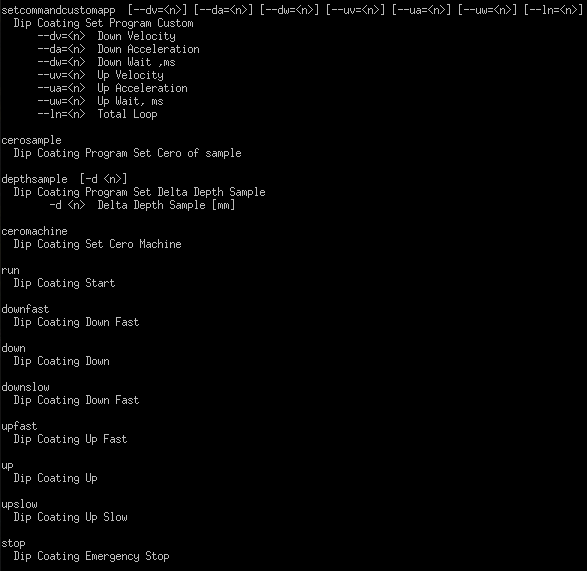
\includegraphics[width=1\textwidth]{./Figures/consola_2.png}
	\caption{Comandos de movimientos.}
	\label{fig:consola_movimientos}
\end{figure}



Para realizar un proceso dip coating a través de la consola se debe seguir el siguiente procedimiento de ejecución de comandos:
\begin{enumerate}
\item Down, up, etc: permiten mover la muestra hasta la posición inicial del experimento.
\item Cerosample: registra la posición.
\item Depthsample: configura la distancia de recorrido de la muestra.
\item Setcommandcustomapp: configura la velocidad y aceleración ascendente y descendente, los tiempos de espera en posición superior e inferior y la cantidad de repeticiones del ciclo.
\item Run: inicia el proceso dip coating.
\item Stop: está disponible para que el usuario pueda detener el proceso.

\end{enumerate}


Se observa en la figura \ref{fig:consola_comandos} la segunda serie de comandos. 

\begin{figure}[h!]
	\centering
	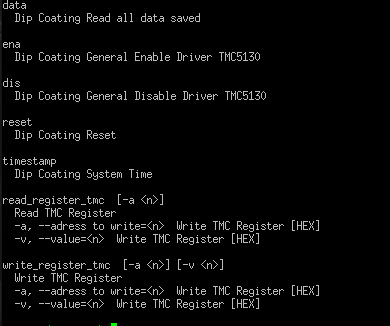
\includegraphics[width=0.7\textwidth]{./Figures/consola_3.png}
	\caption{Comandos de control.}
	\label{fig:consola_comandos}
\end{figure}

Estos comandos permiten utilizar al driver de manera independiente, realizar configuraciones y visualizar el estado de los registros.
Los comandos read-register y write-register sirven para leer y escribir registros sobre el driver TMC5130.

A modo de ejemplo se observa en la figura \ref{fig:comando_lectura} una consulta sobre el registro Xactual[0x21], que expresa la posición actual en micropasos desde la referencia inicial y otra consulta sobre el registro Xtarget[0x2D], cuyo valor expresa la posición objetivo en micropasos que se desea alcanzar. En este ejemplo Xactual = Xtarget ya que el carro estaba detenido. Para ejecutar un movimiento se debe configurar una posición en Xtarget, la misma accionará el motor hasta alcanzar Xactual = Xtarget. Previamente se deben configurar los registros de velocidad y aceleración.


\begin{figure}[h!]
	\centering
	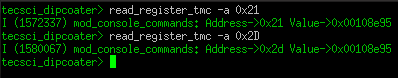
\includegraphics[width=1\textwidth]{./Figures/consola_6.png}
	\caption{Lectura de registros del driver TMC5130.}
	\label{fig:comando_lectura}
\end{figure}


\subsubsection{Pantalla táctil}

La aplicación app hmi establece un canal de comunicación serial entre la pantalla táctil y el microcontrolador, la misma se encarga de procesar datagramas salientes y entrantes. 

En la sección \ref{sec:interfaz_pantalla} se presentó el modelo STWI043WT elegido para el equipo dip coater, el mismo requiere para su configuración el desarrollo de un proyecto con el software \textit{STONE GUI Desing Software}. La interfaz interactiva permite crear pantallas y diferentes tipos de objetos o \textit{widgets} para brindar de funcionalidad a las mismas. El fabricante define también un protocolo de comunicación \citep{web_protocolo_stone} para interaccionar con los objetos que componen cada pantalla.

%\begin{figure}[h!]
%	\centering
%	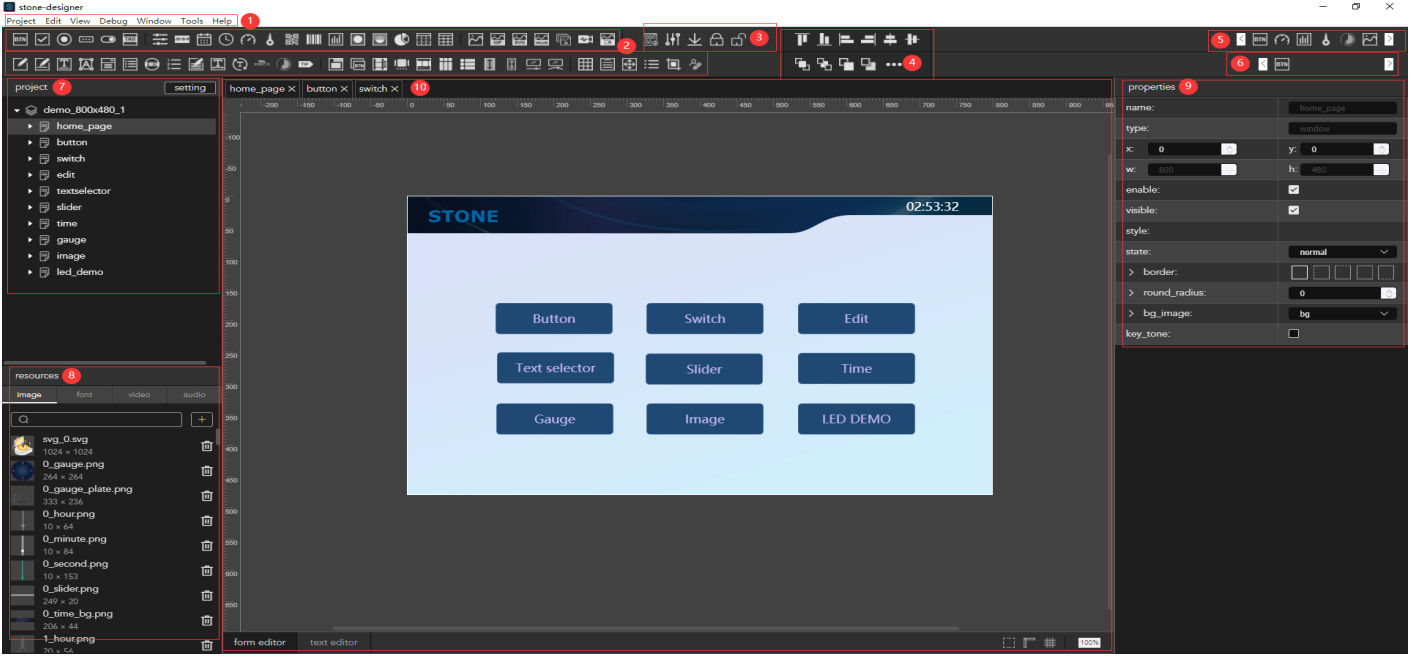
\includegraphics[width=1\textwidth]{./Figures/stone_a.png}
%	\caption{STONE GUI Desing Software.}
%	\label{fig:stone_a}
%\end{figure}



En la figura \ref{fig:datagrama_a} se define el formato de datagrama para enviar datos desde el microcontrolador hacia la pantalla. 

\begin{figure}[h!]
	\centering
	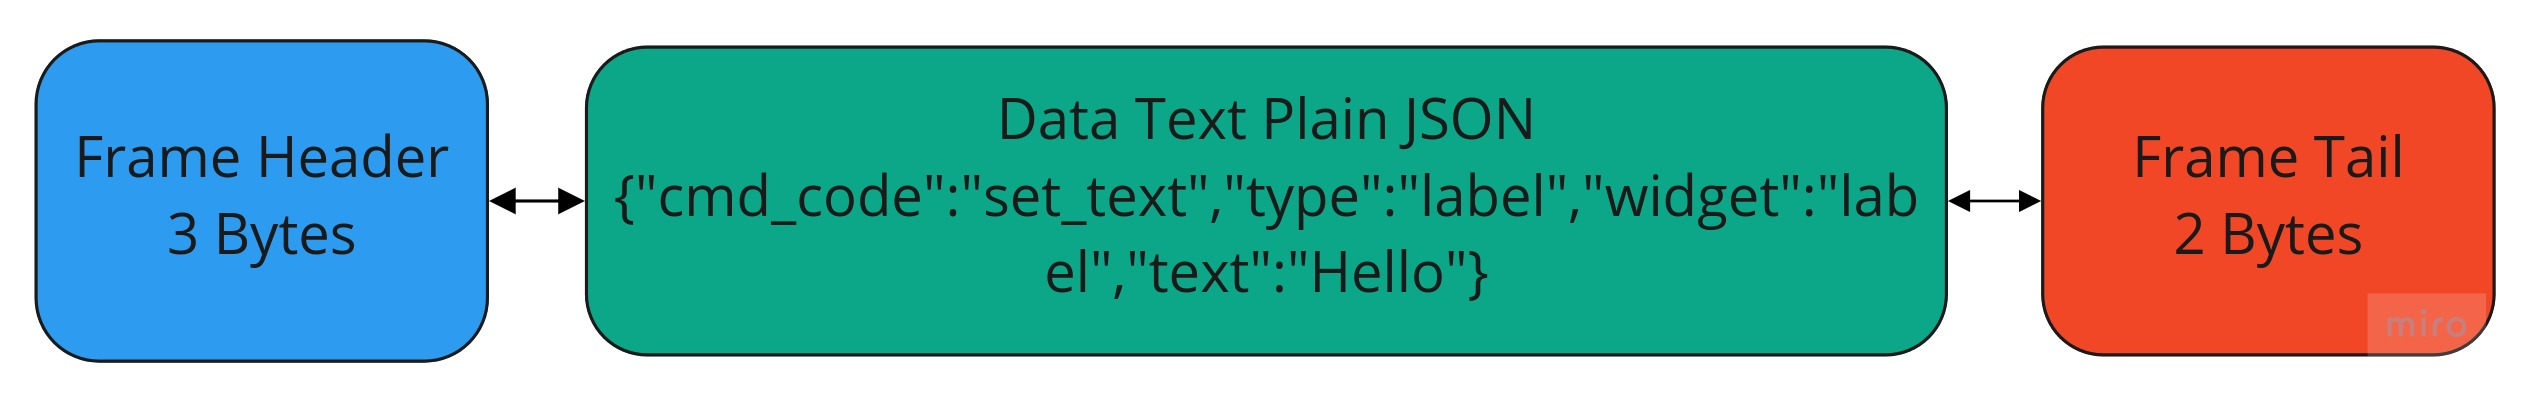
\includegraphics[width=1\textwidth]{./Figures/datagrama_b.jpg}
	\caption{Datagrama desde microcontrolador hacia pantalla.}
	\label{fig:datagrama_b}
\end{figure}

El datagrama está compuesto por tres bloques:
\begin{enumerate}
\item Frame header: 3 bytes fijos.
\item Data: Datos definidos en texto plano con formato \textit{JSON (JavaScript Object Notation)}.
\item Frame tail: 2 bytes fijos.
\end{enumerate}

El campo data define múltiples categorías, se mencionan a continuación las mas importantes:
\begin{itemize}
\item Cmd-code: Es un identificador único que define la instrucción.
\item Type: Define el tipo de objeto.
\item Widget: Define el nombre único del objeto.
\item Text: Define el contenido del objeto, varia según el tipo de objeto.
\end{itemize}  

En la figura \ref{fig:datagrama_a} se define el formato de datagrama para enviar datos desde la pantalla hacia el microcontrolador. El datagrama esta compuesto por los siguientes bloques:

\begin{figure}[h!]
	\centering
	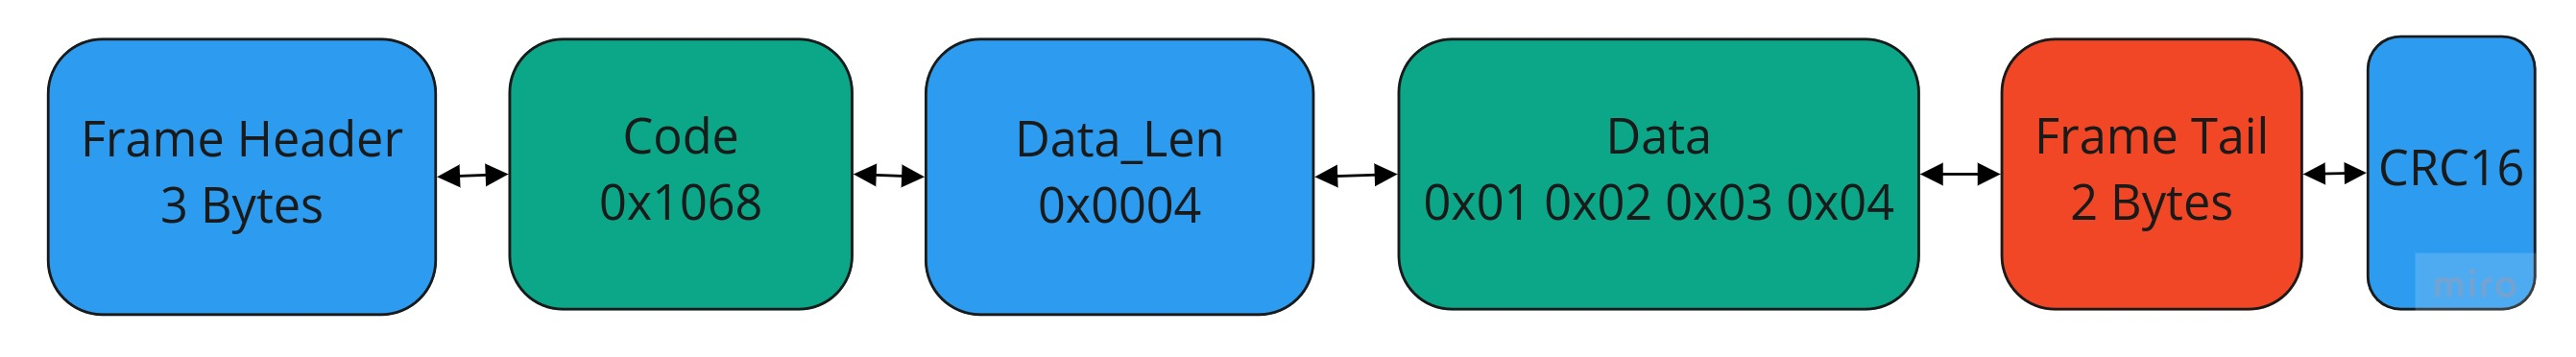
\includegraphics[width=1\textwidth]{./Figures/datagrama_a.jpg}
	\caption{Datagrama desde pantalla hacia microcontrolador.}
	\label{fig:datagrama_a}
\end{figure}

\begin{enumerate}

\item Frame header: 3 bytes fijos.
\item Code: Identificación única de objeto.
\item Data-Len: Define el largo del dato a transmitir.
\item Data: Su tamaño debe coincidir con el item anterior.
\item Frame tail: 2 bytes fijos.
\item CRC16: Para verificación de integridad del datagrama.

\end{enumerate}

Para procesar los datagramas entrantes se implementó un bloque de código que analiza el buffer del periférico UART-1. Cuando hay datos disponibles el periférico envía un evento a través de una \textit{queue} de freeRTOS. El evento UART-DATA se recibe en la \textit{task} mod-hmi-RX-task-loop la cual comienza a procesar dichos datos mientras estén disponibles. En la figura \ref{fig:secuencia_a} se observa el control que se va realizando a cada unos del los bytes entrantes. Si el datagrama pasa todas las condiciones es aceptado y enviado a la \textit{task} app hmi task a través de una \textit{queue} para ser procesado.


\begin{figure}[h!]
	\centering
	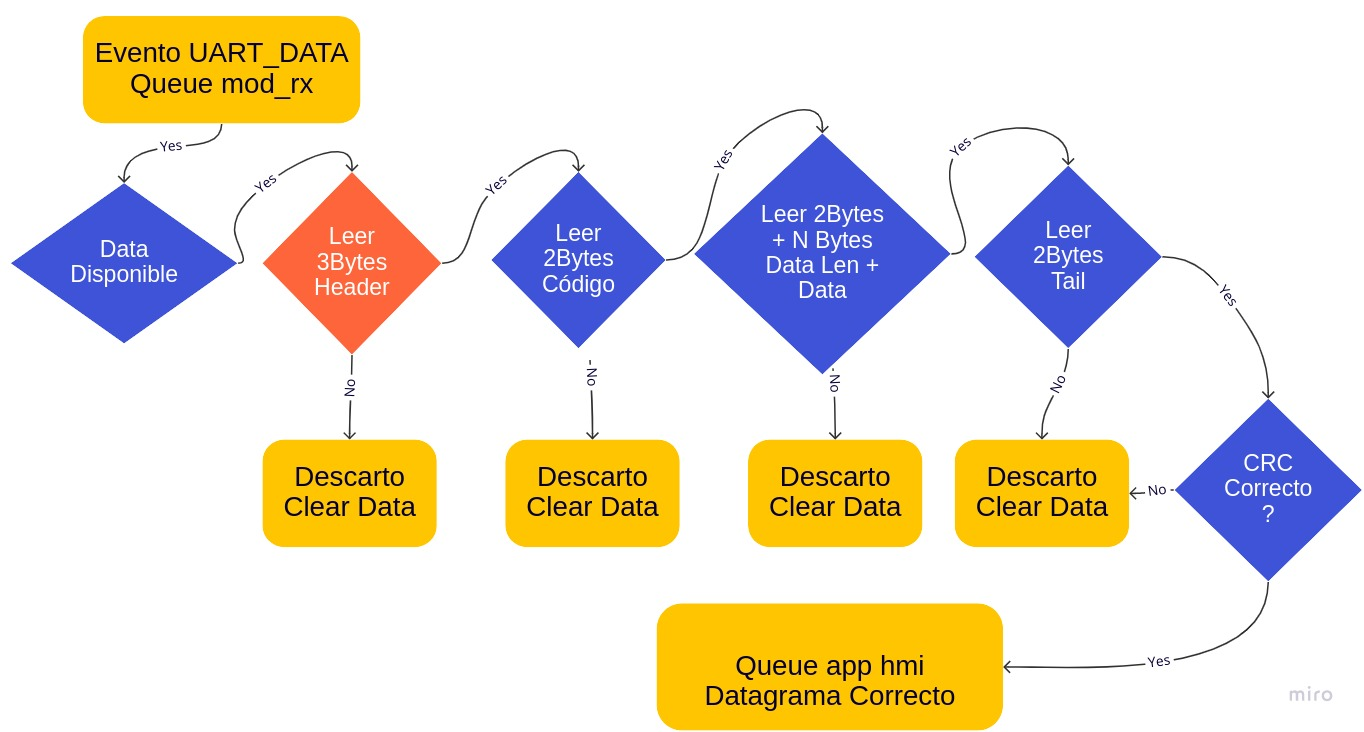
\includegraphics[width=\textwidth]{./Figures/Secuencia_lectura_uart.jpg}
	\caption{Secuencia de procesamientos de datos entrantes.}
	\label{fig:secuencia_a}
\end{figure}

 
En la figura \ref{fig:stone_a} se presenta la pantalla de configuración de programa creada con el software de diseño. 

\begin{figure}[h!]
	\centering
	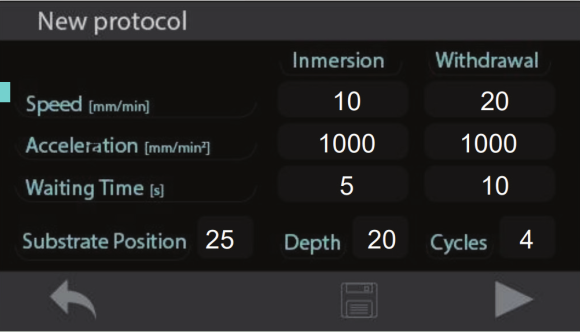
\includegraphics[width=0.7\textwidth]{./Figures/pantalla.png}
	\caption{Pantalla de configuración de programa.}
	\label{fig:stone_a}
\end{figure}  

Al ejecutar el botón \textit{play}, la pantalla envía un serie de datagramas con todos los parámetros configurados en la misma, los datagramas son procesados para verificar su validez y enviados hacia app coating para dar inicio al proceso. 
 

\subsubsection{Registros de variables ambientales}

En la sección \ref{sec:sistema_propuesto} se presentó el requerimiento opcional que establece el registro de variables de humedad, presión y temperatura. El interés del cliente se fundamenta en que ciertos experimentos necesitan realizarse particularmente a humedad y temperatura controlada. 

Para el registro de estas variables se incorporó al sistema un sensor BME280, el mismo integra en un solo CI sensores de presión atmosférica, temperatura y humedad relativa. El fabricante ofrece en sus repositorios \citep{web_repositorio_api_bosh} ejemplos de implementaciones y una API para utilizar todas las funcionalidades del CI.

La comunicación entre el sensor y el microcontrolador se realizó a través del protocolo I2C, se incorporó el módulo del software BOARD I2C que se encarga de inicializar el periférico. También se implementó el módulo API BOSH BME, que trabaja con todas las funcionalidades que ofrece el fabricante en su API. En la figura \ref{fig:api_bosh} de observa el flujo de capas desarrollado:

\begin{figure}[h!]
	\centering
	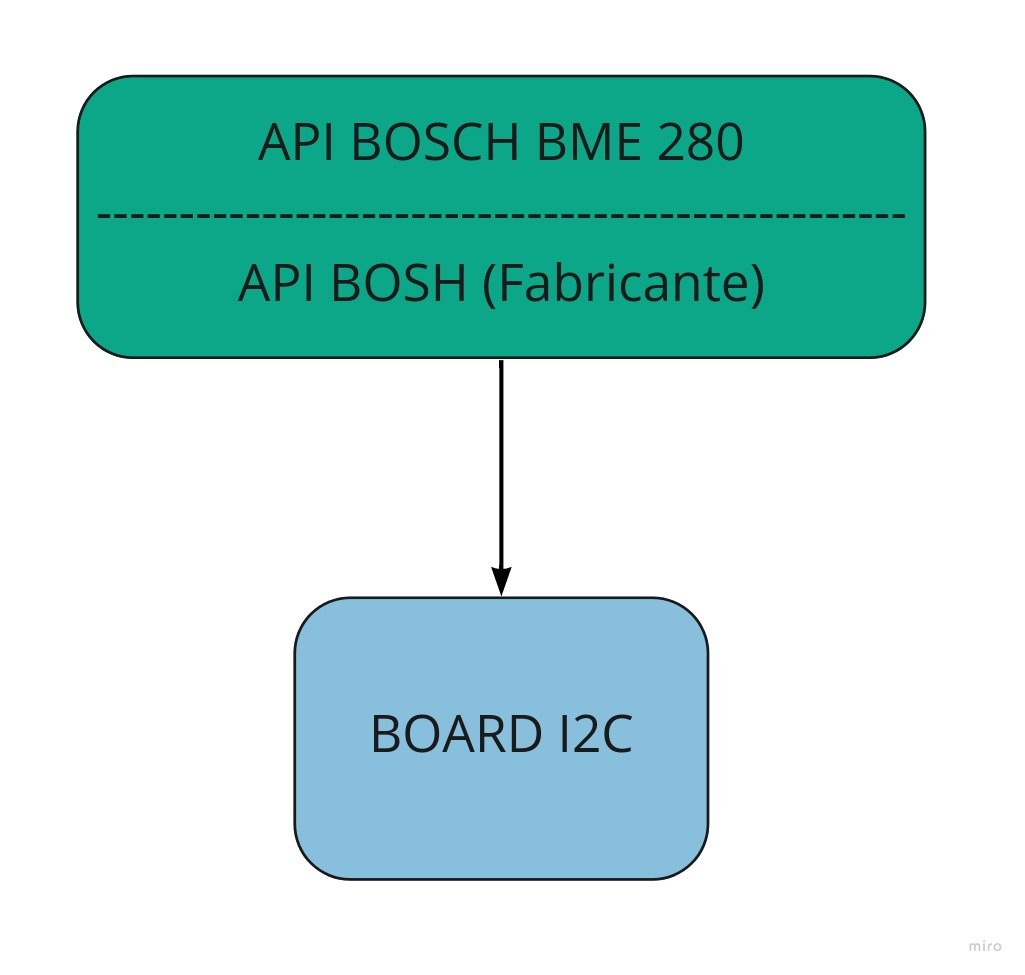
\includegraphics[width=0.4\textwidth]{./Figures/api_bosh_bme.jpg}
	\caption{Módulo API BOSH.}
	\label{fig:api_bosh}
\end{figure}

API BOSH BME inicializada una estructura donde define los siguientes parámetros de interés:
\begin{itemize}
\item Dirección del dispositivo I2C.
\item Función de lectura.
\item Función de escritura.
\item Función de delay.
\item Configuración de modo normal de funcionamiento del sensor. 
\end{itemize}

Para visualizar los datos registrados por el sensor se implementó sobre la APP TEST una rutina de consulta con llamado a funciones de la capa API BOSH BME, se observa en la siguiente figura \ref{fig:api_bosh_consola} los datos registrados en consola.

\begin{figure}[h!]
	\centering
	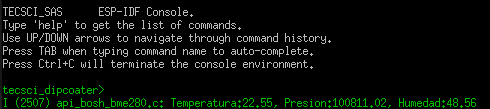
\includegraphics[width=1\textwidth]{./Figures/registro_bme.png}
	\caption{Registro de datos en consola.}
	\label{fig:api_bosh_consola}
\end{figure}

 
El desarrollo de este MPV incluyó el registro de variables ambientales pero no un control y corrección de las mismas con un sistema de control. Sin embargo, se pretende ofrecer en un futuro cercano la funcionalidad de cámara de humedad anexada a este MPV.

\subsubsection{Parámetros de calibración}
\label{subsec:calibracion}

La carpeta /components/config contiene tres archivos de configuración importantes:
\begin{itemize}
\item hardware.h: contiene todas las macros referidas a los pines de conexión del modelo de microcontrolador utilizado.
\item os-config.h: contiene las macros de configuración de las tareas y colas de FreeRTOS. Incluye entre otros parámetros el tamaño del stack, la prioridad y el tiempo de ejecución de cada tarea.
\item machine.h: contiene las macros relacionadas con la calibración mecánica del equipo.
\end{itemize}


La macro más importante configurada en el archivo machine.h es MACHINE STEPS PER MILLIMETER, que debe estar perfectamente determinada. En la sección \ref{sec:calibración} se demuestra el procedimiento realizado para obtener su valor. Esta macro define la cantidad de micropasos necesarios para generar el desplazamiento de 1 mm. La misma esta completamente relacionada con el paso del tornillo acoplado al eje del motor. Las unidades de posición son expresados en micropasos, las unidades de velocidad en micropasos sobre segundos y las unidades de aceleración en micropasos sobre segundos al cuadrado. 

Se observa en la figura \ref{fig:unidades}, extraída de la hoja de datos del driver TMC5130, los factores de corrección que deben aplicarse cuando se cuenta con un clock externo incorporado en el circuito electrónico. 

\begin{figure}[h!]
	\centering
	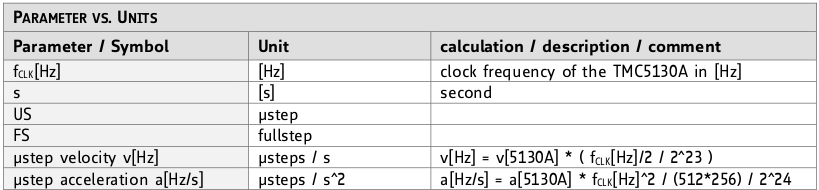
\includegraphics[width=1\textwidth]{./Figures/unit.png}
	\caption{Unidades.}
	\label{fig:unidades}
\end{figure}

Se observa en el fragmento de código \ref{cod:vMachine} el cálculo de las constantes que corrigen los valores de velocidad y aceleración.

%Como se mencionó en la subsección \ref{subsection:Driver TMC5130} el equipo se configuró con 51200 micropasos por vuelta completa.  
 
 

\begin{lstlisting}[label=cod:vMachine,caption=Macros de desplazamiento y factores de corrección.]  % Start your code-block
/*Buscar este numero con calibración mecánica del sistema*/

#define MACHINE_STEPS_PER_MILLIMETER	(12916)		
#define MACHINE_EXT_CLOCK						  (16000000)	//16MHz


/*FACTOR*/
/*((MACHINE_EXT_CLOCK/2)*(1/8388608))*/	
#define MACHINE_USTEPS_VELOCITY_FACTOR	  (0.9536743164)
/*((MACHINE_EXT_CLOCK*MACHINE_EXT_CLOCK)/(512*256)/ (16777216) )*/
#define MACHINE_USTEPS_ACELERATION_FACTOR (116.4153218)


/*UPPER AND LOWER MECHANICAL LIMIT*/

#define UPPER_LIMIT 	(MACHINE_STEPS_PER_MILLIMETER * 10 ) // 10mm
#define LOWER_LIMIT		(MACHINE_STEPS_PER_MILLIMETER * 290) // 290mm

\end{lstlisting}






%----------------------------------------------------------------------------------------
%	SECTION 3
%----------------------------------------------------------------------------------------

\section{Estructura mecánica}
\subsection{Fabricación de piezas personalizadas a través de mecanizado CNC}

\subsubsection{Etapa CAD}

Como se mencionó en la sección \ref{sec:estructura_mecanica} se utilizó para el diseño mecánico del equipo el software BOBCAD. El módulo CAD del software permite realizar modelos 2D y 3D de piezas.

El prototipo dip coater cuenta actualmente con dos piezas mecanizadas en aluminio. Se observa en la figura \ref{fig:carro} la pieza que se acopla al carro de la guiá lineal presentada en la sección \ref{sec:estructura_mecanica}.

\begin{figure}[ht]
	\centering
	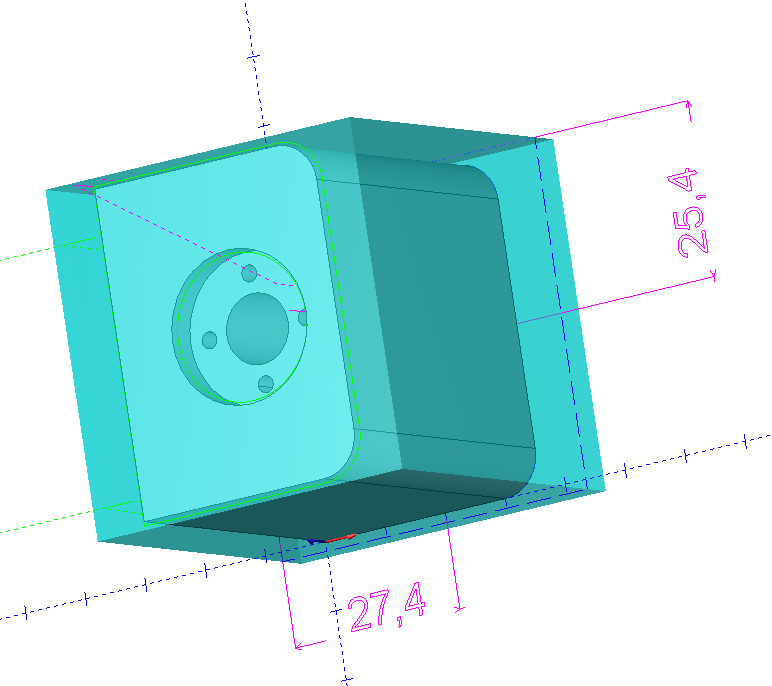
\includegraphics[width=.5\textwidth]{./Figures/3d_carro.png}
	\caption{Pieza personalizada soporte de carro.}
	\label{fig:carro}
\end{figure}

Y en la figura \ref{fig:estructura_superior} el soporte superior que sostiene el motor paso a paso y el  tornillo acoplado al eje del motor.

\begin{figure}[h]
	\centering
	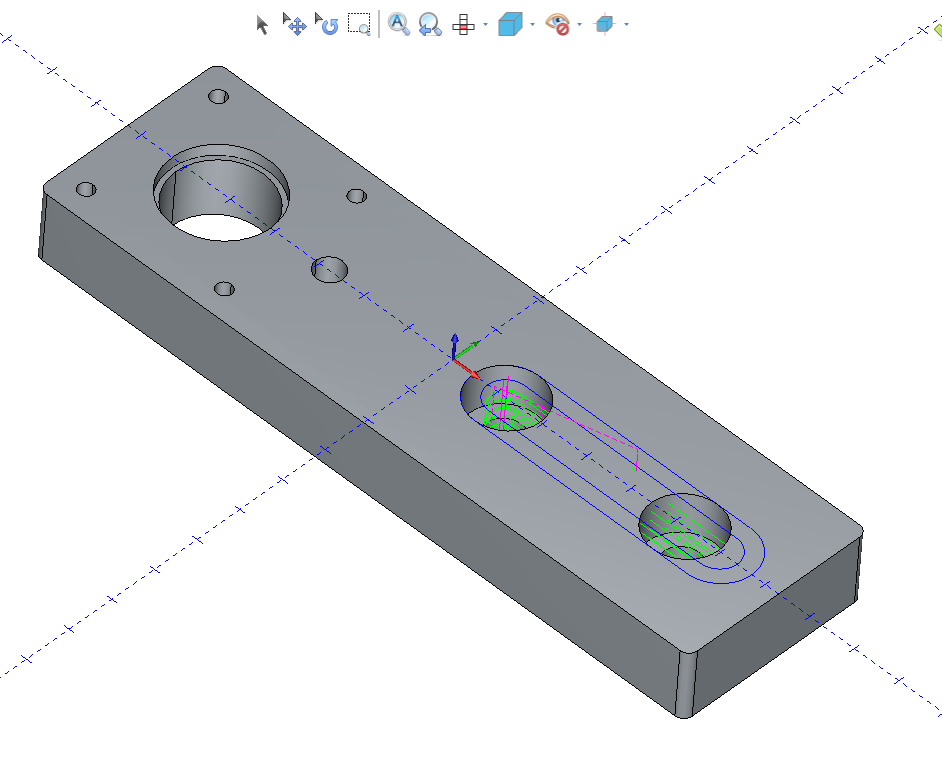
\includegraphics[width=.5\textwidth]{./Figures/3d_top.png}
	\caption{Piezas personalizada soporte de estructura superior.}
	\label{fig:estructura_superior}
\end{figure}

Con los modelos 3D terminados, se fabricó un primer lote utilizando impresión 3D en plástico.
Luego que las piezas fueron probadas, testeadas y aprobadas en el prototipo, se pasó a la fabricación final sobre aluminio.

\subsubsection{Etapa CAM}

La estrategia utilizada en el mecanizado CNC es el método de arranque de viruta. Este consiste en partir de un bloque de aluminio con volumen de material suficiente y desbastar con herramientas de corte hasta modelar la pieza. Esta estrategia se programa en la parte CAM del software. Existen diferentes operaciones de mecanizado que se utilizan según el tipo de pieza que se desee fabricar. Tal es el caso de refrentado, vaciado, fresado de chaflán, taladrado y roscado entre otras. Cada una de estas operaciones  en general se realizan con herramientas específicas que son definidas en la configuración del software.

A modo de ejemplo se presenta en la figura \ref{fig:estrategia} el listado de operaciones realizadas para la fabricación de la pieza soporte carro del equipo.

\begin{figure}[h]
	\centering
	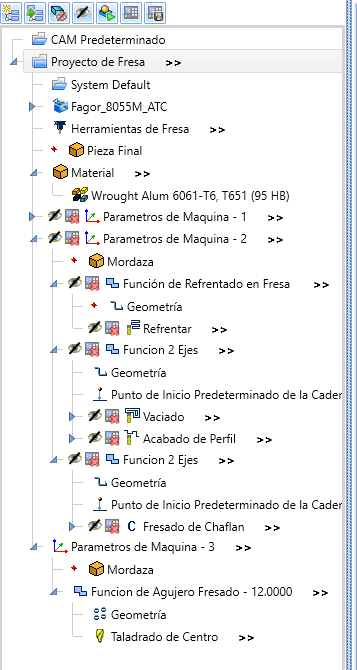
\includegraphics[width=.6\textwidth]{./Figures/3d_estrategia.png}
	\caption{Operaciones de mecanizado en software Bodcad.}
	\label{fig:estrategia}
\end{figure}

En general las piezas se fabrican en dos etapas, primero a través de diferentes operaciones se mecaniza la parte superior, luego se rota la pieza 180° y se mecaniza la parte inferior.


El material mecanizado para la fabricación de estas piezas fue aluminio 6061, el mismo es una aleación endurecida compuesta por aluminio, magnesio y silicio. La elección se basó en que el mismo puede someterse a tratamientos de anodizado posteriores. El anodizado es un tratamiento electrolítico, que genera una capa superficial de óxido de aluminio (alúmina). De espesor superior que el aluminio en estado natural, tiene como ventajas la protección contra atmósferas agresivas, agentes químicos y una mayor dureza superficial.

Finalmente en la figura \ref{fig:real_custom} se observan ambas piezas fabricadas.

\begin{figure}[h]
	\centering
	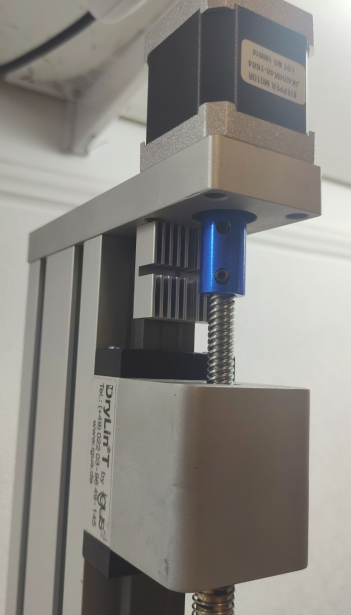
\includegraphics[width=0.5\textwidth]{./Figures/real_custom.png}
	\caption{Piezas fabricadas en centro de mecanizado.}
	\label{fig:real_custom}
\end{figure}


\subsection{Modelos 3D y real}

En la figura \ref{fig:mecanica_3d_model} se presenta el primer modelo 3D diseñado del equipo dip coater.
\begin{figure}[h]
	\centering
	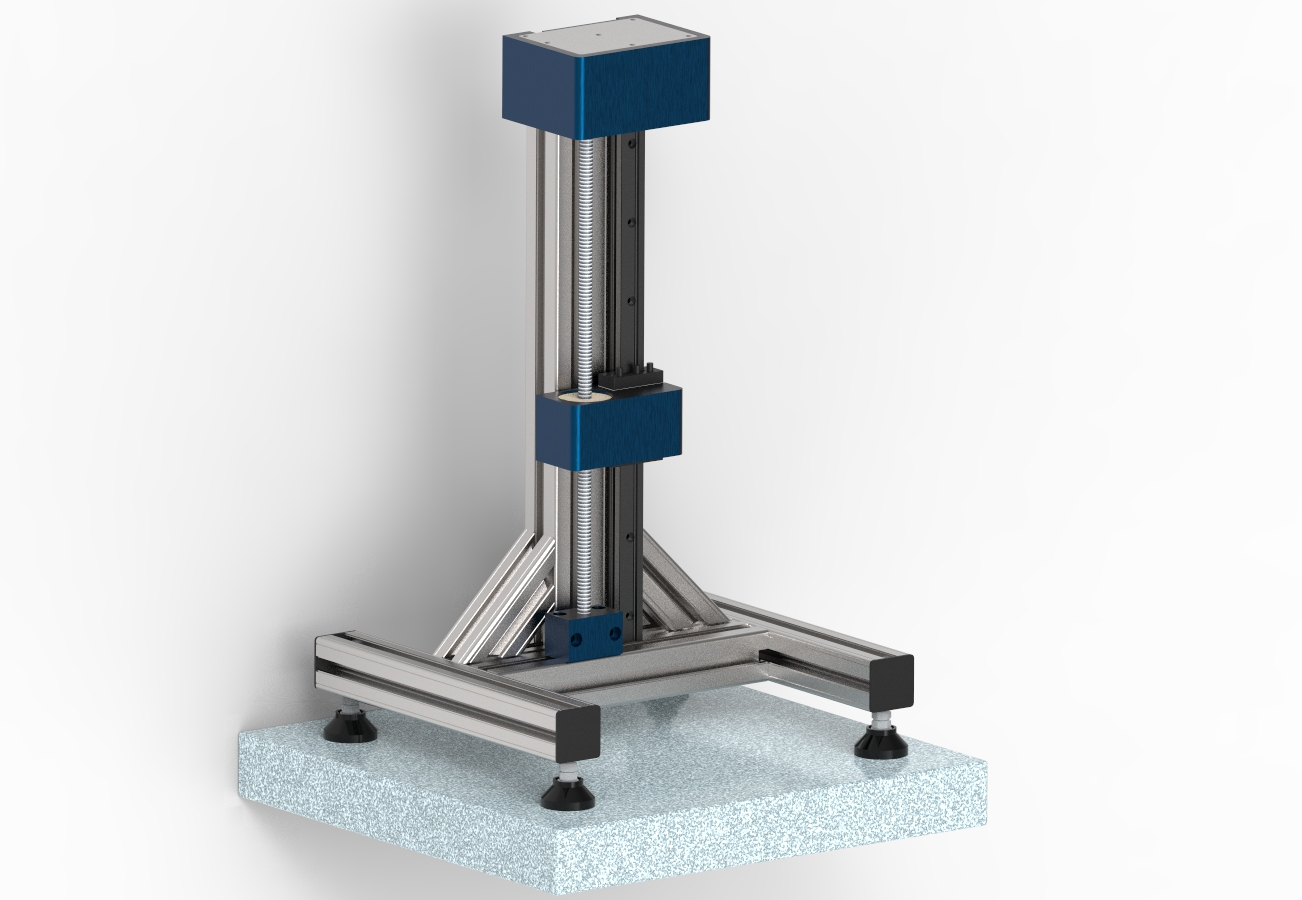
\includegraphics[width=0.9\textwidth]{./Figures/3d.jpg}
	\caption{Modelo 3D.}
	\label{fig:mecanica_3d_model}
\end{figure}


%Se detallan a continuación los siguientes componentes fundamentales del equipo:
%\begin{itemize}
%\item Guiás lineales IGUS 
%\item Mecanizado soporte superior y mecanizado carro
%\item Placa electrónica
%\item Pantalla táctil 4.3 inch
%\end{itemize}

Luego de sucesivas iteraciones con pruebas de piezas impresas en material plástico se logró fabricar un primer prototipo completamente en metal que se presenta en la figura \ref{fig:mecanica_real_model}.

\begin{figure}[h]
	\centering
	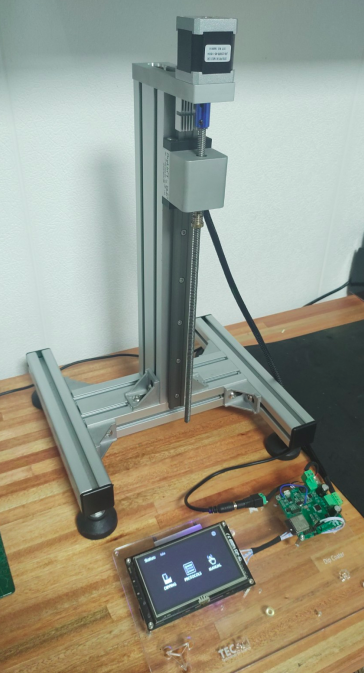
\includegraphics[width=0.4\textwidth]{./Figures/real.png}
	\caption{Primer prototipo dip coater TECSCI.}
	\label{fig:mecanica_real_model}
\end{figure}

